\documentclass{article}

\usepackage[english]{babel}
\usepackage{amsthm,amsmath,lipsum}
\usepackage[algo2e]{algorithm2e} 
\usepackage{xcolor}
\usepackage{fullpage}
\usepackage{amssymb}
\usepackage{centernot}
%\usepackage{authblk}
\usepackage{tikz}
\usepackage{soul}
\usetikzlibrary{shapes.geometric, arrows}
\usetikzlibrary{positioning}
\usetikzlibrary{calc}


\DeclareFontFamily{U}{mathb}{\hyphenchar\font45}
\DeclareFontShape{U}{mathb}{m}{n}{
      <5> <6> <7> <8> <9> <10> gen * mathb
      <10.95> mathb10 <12> <14.4> <17.28> <20.74> <24.88> mathb12
}{}
\DeclareSymbolFont{mathb}{U}{mathb}{m}{n}
\DeclareMathSymbol{\llcurly}{3}{mathb}{"CE}
\DeclareMathSymbol{\ggcurly}{3}{mathb}{"CF}


\usepackage{thm-restate}




\theoremstyle{plain}

\newtheorem{example}{Example}
\newtheorem{theorem}{Theorem}
\newtheorem{lemma}{Lemma}
\newtheorem{definition}{Definition}
\newtheorem{observation}{Observation}
\newtheorem{corollary}{Corollary}
\newtheorem{claim}{Claim}


\usepackage{times}
\usepackage{soul}
\usepackage{url}
\usepackage[hidelinks]{hyperref}
\usepackage[utf8]{inputenc}
\usepackage[small]{caption}
\usepackage{graphicx}
\usepackage{amsmath}
\usepackage{amsthm}
\usepackage{amssymb}
\usepackage{booktabs}
\usepackage{booktabs}
\usepackage{algorithm}
\usepackage{algorithmic}
\usepackage{color}
\usepackage[switch]{lineno}

\urlstyle{same}
\usepackage[most]{tcolorbox}










\title{Maximin Share Guarantees for Few Agents with Subadditive Valuations}



\author{George Christodoulou\thanks{Aristotle University of
    Thessaloniki, and Archimedes/Athena RC, Greece. Email: \texttt{\{gichristo,vgchrist,smastra\}@csd.auth.gr} }
\and{Vasilis Christoforidis\footnotemark[1]}
\and {Symeon Mastrakoulis\footnotemark[1]}
\and Alkmini Sgouritsa\thanks{Athens University of Economics and Business, and Archimedes/Athena RC, Greece. Email: \texttt{alkmini@aueb.gr}}}

%\affil[1]{Aristotle University of
 %   Thessaloniki and Archimedes/Athena RC, Greece.}  
%\affil[2]{Athens University of Economics and Business, and Archimedes/Athena RC, Greece.}
\date{}



\begin{document}

\maketitle

\begin{abstract}
    We study the problem of fairly allocating a set of indivisible items among a set of agents. We consider the notion of (approximate) maximin share (MMS) and we provide an improved lower bound of $1/2$ (which is tight) for the case of subadditive valuations when the number of agents is at most four. We also provide a tight lower bound for the case of multiple agents, when they are equipped with one of two possible types of valuations. Moreover, we propose a new model that extends previously studied models in the area of fair division, which will hopefully give rise to further research. We demonstrate the usefulness of this model by employing it as a technical tool to derive our main result, and we provide a thorough analysis for this model for the case of three agents. Finally, we provide an improved impossibility result for the case of three submodular agents. 
    
\end{abstract}
\usetikzlibrary {patterns,patterns.meta}
% 
% 
The widespread integration of communication networks and smart devices in modern control systems has increased the vulnerability of industrial systems to online cyber-attacks, e.g., Industroyer, Blackenergy, etc \citep{osti_1505628}.
% Modern control systems have seen a large push to include communication networks and smart devices to increase performance, made possible by improvements in communication device cost and energy consumption. This trend has been coupled with the usage of open-standard communication protocols among industrial control systems, making them vulnerable to online cyber-attacks such as Industroyer, Blackenergy, etc \citep{osti_1505628}. 
To counter this, methods have been developed to improve security by achieving attack detection, mitigation, and monitoring, among others \citep{sandberg2022secure}. This paper focuses on active attack diagnosis to mitigate stealthy attacks. 
%
%\subsection{Literature review}

Active diagnosis techniques rely on the inclusion of additional moduli to control systems
% inclusion within the control system of additional moduli 
to alter the behavior of the system compared to information known by the attacker. 
For instance, the concept of additive watermarking was introduced in \cite{mo2015physical}, where noise signals of known mean and variance are added at the plant and compensated for it at the controller. 
This compensation, however, is not exact, causing some performance degradation. Thus, trade-offs between performance and detectability  are necessary \citep{zhu2023detection}.
% A later work \citep{zhu2023detection} designs the watermark signal by trading performance for detection. Thus, although additive watermarking serves as a good detection scheme, they endure performance losses even in the nominal case. 

In encrypted control \citep{darup2021encrypted}, the sensor data is encrypted, sent to the controller, and then operated on directly. Encrypted input signals are sent back to the plant for decryption. Although encryption is widespread in IT security, in control systems it presents some concerns, such as the introduction of time delays \citep{stabile2024verifiable}, while it may present inherent weaknesses \citep{alisic2023model}.
% they are not preferred as they introduce time delays \citep{stabile2024verifiable} which can cause instability, and some encryption schemes can be very weak  \citep{alisic2023model}. 

In moving target defense \citep{griffioen2020moving}, the plant is augmented with fictitious dynamics, known to the controller. The plant output is transmitted to the controller along with the fictitious states over a network under attack. 
The additional measurements then aide in the detection of attacks. 
This comes at the cost of higher communication bandwidth needs, which increases rapidly with the dimension of the augmented systems.
% Since the dynamics of the fictitious dynamics are exactly known to the controller, the attack is detected easily. However, when the scale of the system increases, the communication bandwidth used by moving the target defense approach increases rapidly. 

Other recently proposed works include two-way coding \citep{fang2019two}, a weak encryuption technique, and dynamic masking \citep{abdalmoaty2023privacy}, which enhances privacy as well as security, have been shown to be effective against zero-dynamics attacks.
% Two-way coding \citep{fang2019two} and dynamic masking \citep{abdalmoaty2023privacy} are other recently proposed approaches. Two-way coding is another form of weak encryption technique whilst dynamic masking proposes an architecture that enhances both privacy and security. These schemes are shown to be effective against zero dynamics attacks but remain to be studied for other classes of attacks. 
% Recent extensions include \citep{mukherjee2021secure,ramos2024privacy}.
% Some other works which are related are \citep{mukherjee2021secure}, an extension of \cite{fang2019two}. The work \citep{ramos2024privacy} is an extension of moving target defense for multi-agent systems. 
Furthermore, filtering techniques for attack detection are proposed by \cite{murguia2020security,hashemi2022codesign,escudero2023safety}, while not focusing on stealthy attacks.
% The works \citep{murguia2020security,hashemi2022codesign,escudero2023safety} develop filtering techniques to guarantee safety, without being focused on stealthy covert attacks.

Multiplicative watermarking (mWM) has been proposed by the authors as a diagnosis technique \citep{ferrari2020switching}. mWM consists of a pair of filters on each communication channel between the plant and its controller; the scheme is affine to weak encryption, whereby ``encoding'' and ``decoding'' are done by changing signals' dynamic characteristics through inverse pairs of filters. This enables original signals to be recovered exactly, and thus does not lead to performance degradation.
% A multiplicative watermark is an affine to a weak encryption technique, through which the signal is ``encoded'' by a filter, changing its dynamic behavior. The use of inverse pairs means that the original signal can be recovered, through ``decoding'' via an inverse filter. As such, differently to techniques based on additive watermarking, no performance is lost due to the injection of noise, and there are no bandwidth limitations.

%\subsection{Contributions}
One of the critical features of multiplicative watermarking is that to detect stealthy attacks, the mWM filter parameters must be switched over time. In this paper, an algorithm to optimally design the mWM parameters after a switching event is presented, enhancing detection performance, without changing the switching time.
% This is done without changing the switching time, which is taken as given.

\textcolor{black}{
To formalize the filter design problem, we suppose the defender is interested in optimal performance against adversaries injecting covert attacks with matched system parameters \citep{smith2015covert}, including the mWM parameters prior to the switch. This scenario represents a worst case where malicious agents can take full control of the system while remaining undetected.
Thus, the attack strategy is explicitly included within the formulation of the closed-loop system, and the mWM filters are chosen by solving an optimization problem minimizing the attack-energy-constrained output-to-output gain (AEC-OOG) \citep{anand2023risk}, a variation of the output-to-output gain proposed in  \cite{teixeira2015strategic}.
}
The main contributions of this paper are:
% We consider an adversary injecting a covert attack with matched system parameters \citep{smith2015covert}, i.e., an attacker with full knowledge of the control system parameters, including those of the mWM filters before the switch. This scenario is taken as a worst case, as it has been shown that this class of attacks can be made stealthy. To quantitatively define a cost, the output-to-output gain (OOG) \citep{teixeira2015strategic} is leveraged,
% a metric introduced to evaluate the impact of an additive attack in a control system. %Specifically, OOG evaluates the worst-case performance loss that an attacker injecting an undetectable attack can obtain. 
% Here, the maximum performance loss caused by a stealthy adversary with limited energy is taken, the attack-energy-constrained OOG (AEC-OOG) \citep{anand2023risk}. The main contributions of this paper are:
\begin{enumerate}
%[label=\alph*.]
\item The problem of optimally designing the switching mWM filters is formulated as an optimization problem, with the AEC-OOG is taken as the objective;%where the AEC-OOG is taken as the impact metric; 
\item The worst-case scenario of a covert attack with exact knowledge of plant and mWM filter parameters is embedded within the design problem;
% The optimization problem is defined to incorporate the worst-case scenario of a covert attack with exact knowledge of plant and mWM filter parameters;
\item The feasibility of the optimization problem is shown to be dependent only on stability conditions; 
\item A solution scheme is proposed to promote randomization of the mWM filter parameters such that an eavesdropping adversary cannot remain stealthy.
\end{enumerate} 

This builds on the results of \cite{ferrari2020switching}, where the focus was on the design of the switching protocols, rather than the parameters themselves.
Compared to previous work \citep{gallo2021design}, this paper introduces an optimization problem which is always feasible (thanks to the use of AEC-OOG in the objective), while also considering a more sophisticated class of covert attacks, where the presence of watermark is known to the adversary. 
Moreover, this paper poses a different objective than \citep{zhang2023hybrid}; indeed, while \citep{zhang2023hybrid} provided a design strategy to ensure certain privacy properties, in this paper we address the problem of optimal parameter design following a switching event.


%\subsection{Organization}
The rest of the paper is organized as follows. 
After formulating the problem in Section~\ref{sec:PF}, we propose our design algorithm in Section~\ref{sec:main}, and analyze its properties. It is then evaluated through a numerical example in Section~\ref{sec:NE}, and concluding remarks are given Section~\ref{sec:Con}.
% We provide the problem background in Section~\ref{sec:PF}. We formulate the design problem in Section~\ref{sec:main}, together with an analysis of its properties. The proposed algorithm is evaluated through a numerical example in Section \ref{sec:NE}. Concluding remarks are offered in Section \ref{sec:Con}.

 \subsection{Our contribution}

We study the existence of approximate MMS allocations, a predominant notion of fairness in settings with indivisible goods, under submodular
and subadditive valuations. We focus on settings with few agents. We are able to show the following results.

\begin{itemize}
    \item In our main technical result (Theorem~\ref{thm:mainTheorem}), we show the existence of $1/2$-MMS allocations for at most four agents with subadditive valuations. We note that this result improves the best known bounds for many other valuation classes, including OXS, Gross Substitutes, submodular and XOS. We emphasize that the guarantee of our theorem matches the best known impossibility result due to \cite{GhodsiHSSY22}, thus settling the case of four agents for both subbaditive and XOS valuations (see also Table~\ref{table:Results}). 

    \item We show the existence of $1/2$-MMS allocations for multiple agents when they have one of two admissible valuation functions (Theorem~\ref{thm:two-types}).

    
    \item On the way to prove Theorem~\ref{thm:mainTheorem} we develop a new model that is useful for inductive arguments. This model incorporates nicely previously studied MMS variants, and we believe that it is of independent interest. In Section~\ref{sec:Reductions}, we provide a thorough study of approximate guarantees for three agents and we are able to provide two complete characterizations: one for the case of $1/2$-MMS$(\mathbf{d})$ (Theorem~\ref{thm:three-general}) and one for the case of $(1,1/2,1/2)$-MMS$(\bf d)$ (Theorem~\ref{thm:three-general-approximate}). 

    \item We show an improved impossibility result for three agents with submodular valuation functions: we present an instance in which an $\alpha$-MMS allocation does not exist for $\alpha > 2/3$ (Theorem~\ref{thm:SubmodUB}). This improves the previous best known result of 3/4 due to \cite{GhodsiHSSY22}.

    
\end{itemize}




 \section{System Overview}
\label{sec:overview}

In this section, we present the control system architecture of the proposed framework, shown in Fig. \ref{fig:controlArchi}. 
Empirically, humanoid kino-dynamics MPC explicitly optimizes the joint states through kinematics constraints \cite{gu2025humanoid}, while traditional centroidal-dynamics MPC often requires subsequent inverse kinematics solver or whole-body control for motion execution. Both approaches employ nonlinear approaches to solve the optimization problem. In our framework, we proposed a Gait-Net-augmented sequential CMPC algorithm that translates the original nonlinear problem into convex sequential subproblems. With the additional assistance of Gait-Net, we reduce the optimization variable and mimic a natural step duration decision in each iteration. 

The control framework converts user commands and contact sequence into joint space references $\{\mathbf q_k^\text{ref} \in \mathbb R^{6+n_j},\: \dot{\mathbf q}_k^\text{ref} \in \mathbb R^{6+n_j}\}^h_{k = 0}$ and foot location reference trajectory $\{\bm p_f^\text{ref}\in \mathbb R^{3n_i}\}^h_{k = 0}$, where $n_j$ is the number of joints, $n_i$ is the number of contact/foot, and $h$ is a finite number of horizon. These joint-space trajectories, along with joint-space feedback states, are then translated into spatial momenta $\bm h\in \mathbb R^6$ and their primitive, the centroidal pose $\bm H\in \mathbb R^6$, which are the state variables used in the Gait-Net-augmented kino-dynamic MPC. Within the MPC, we break down the nonlinear dynamics constraints into sequential CMPC subproblems that can be solved through QP solvers. In each sequential iteration $j$, the Gait-Net predicts and updates the MPC sampling time $dt$ towards convergence and enables variable-frequency walking.
The spatial momentum and pose trajectories are updated at each iteration to reflect the kinematic configuration based on the iterative solution of $dt$, CoM location $\bm p_c \in \mathbb R^3$, and foot locations $\bm p_f\in \mathbb R^{3n_i}$,
providing a kinematically feasible reference. Once the terminal condition is met in the custom sequential solver, the control inputs are then mapped to motor commands in low-level control, which incorporates standard techniques such as inverse kinematics, contact Jacobian mapping, and joint-PD swing leg control \cite{di2018dynamic}. Notably, the full Gait-Net-augmented Kino-dynamic MPC is run at the beginning of each footstep to determine the step duration, the rest of the duration will incorporate the kino-dynamic MPC with the same MPC $dt$ throughout this very footstep. 


 


 \section{Related Work}
\subsection{Multimodal Large Language Models}
% Building on the success of large language models (LLMs) \citep{yao2024tree, glm2024chatglm, achiam2023gpt, touvron2023llama, brown2020language}, multimodal large language models (MLLMs) \citep{liu2024improved, li2023blip, zhu2023minigpt, wang2023cogvlm, liu2024visual} extend these capabilities by integrating vision and text processing, achieving remarkable performance in tasks involving images, videos, and multimodal reasoning. However, handling visual data poses computational challenges due to the redundancy and low information density of high-resolution tokens \citep{liang2022evit} and the quadratic scaling of attention mechanisms \citep{vaswani2017attention}.
% For instance, models like LLaVA \citep{liu2023improvedllava} and mini-Gemini-HD \citep{li2024mini} encode high-resolution images into thousands of tokens, while video-based models such as VideoLLaVA \citep{lin2023video} and VideoPoet \citep{kondratyuk2023videopoet} allocate even more tokens to process multiple frames. These challenges highlight the need for more efficient token representations and longer context lengths to enable scalability. Recent advancements, such as Gemini \citep{geminiteam2023gemini} and LWM \citep{liu2024world}, have focused on addressing these issues by optimizing token efficiency and extending the context length, paving the way for more scalable and effective MLLMs.

The remarkable success of large language models (LLMs) \citep{radford2019language, brown2020language} has spurred a growing trend of extending their advanced reasoning capabilities to multi-modal tasks, leading to the development of vision-language models (VLMs) \citep{huang2023languageneedaligningperception, driess2023palmeembodiedmultimodallanguage, liu2024visual, Qwen-VL}. These VLMs typically consist of a visual encoder \citep{radford2021learning} that serializes input image representations and an LLM responsible for text generation. To enable the LLM to process visual inputs, an alignment module is employed to bridge the gap between visual and textual modalities. This module can take various forms, such as a simple linear layer, an MLP projector, or a more complex query-based network. While this integration allows the LLM to gain visual perception, it also introduces significant computational challenges due to the long sequences of visual tokens.

Moreover, existing VLMs often exhibit limitations, such as visual shortcomings or hallucinations, which hinder their performance. Efforts to enhance VLM capabilities by increasing input image resolution have further exacerbated computational demands. For instance, encoding higher-resolution images results in a substantial increase in the number of visual tokens. A model like LLaVA-1.5 \citep{liu2024improved} generates 576 visual tokens for a single image, while its successor, LLaVA-NeXT \citep{liu2024llavanext}, produces up to 2880 tokens at double the resolution, far exceeding the length of typical textual prompts.
Optimizing the inference efficiency of VLMs is thus a critical task to facilitate their deployment in real-world scenarios with limited computational resources.

\subsection{Visual Token Compression}
% Visual tokens often exceed text tokens by tens to hundreds of times, with visual signals being more spatially redundant compared to information dense text \citep{marr2010vision}.
% Various methods have been proposed to address this issue. For instance, LLaMA-VID \citep{li2023llama} uses a Q-Former with context tokens, and DeCo \citep{yao2024deco} applies adaptive pooling to downsample visual tokens at the patch level.
% However, these approaches require modifying model components and additional training, increasing computational and training costs.
% ToMe~\citep{bolya2022tome} reduces tokens without training by adding a token merge module to ViTs, but this disrupts early cross-modal interactions in language models~\citep{xing2024PyramidDrop}. FastV~\citep{chen2024image} selects important visual tokens using attention scores, while SparseVLM~\citep{zhang2024sparsevlm} incorporates text guidance via cross-modal attention.
% However, these methods forgo flash-attention~\citep{dao2022flashattention, dao2023flashattention2} and primarily focus on token importance, overlooking the impact of token duplication.
% In our work, we preserve hardware acceleration compatibility, including flash attention, while considering both token importance and duplication for token reduction.

Visual tokens are often significantly more numerous than text tokens, with higher spatial redundancy and lower information density. To address this issue, various methods have been proposed for reducing visual token counts in vision language models. For instance, some approaches modify model components, such as using context tokens in Q-Former \citep{li2023llama} or applying adaptive pooling at the patch level, but these typically require additional training and increase computational costs. Other techniques, like Token Merging (ToMe) \citep{bolya2022tome} and FastV \citep{chen2024image}, focus on reducing tokens without retraining by merging tokens or selecting important ones based on attention scores. SparseVLM \cite{zhang2024sparsevlm} incorporates text guidance through cross-modal attention to refine token selection. However, these methods often overlook hardware acceleration compatibility and fail to account for token duplication alongside token importance. Furthermore, while token pruning has been extensively explored in natural language processing and computer vision to improve inference efficiency, its application to VLMs remains under-explored. Existing pruning strategies, such as those in FastV and SparseVLM, rely on text-visual attention within large language models (LLMs) to evaluate token importance, which may not align well with actual visual token relevance.



 In this section,  we introduce related concepts including GNN for recommendation, negative sampling, and Mixup \cite{mixup}.

\subsection{Graph Neural Networks for Recommendation}
 Recommendation is the most important technology in many e-commerce platforms, which has evolved from collaborative filtering to graph-based models. Graph-based recommendation represents all users and items by embedding and recommending items with maximum similarity score (by a inner product operation) for a given user. Here, we briefly describe the pipeline of GNN-based representation learning, including aggregation and optimization with negative sampling.

GNNs learn distributed vectors of nodes by leveraging node features and the graph structure. 
The neighborhood aggregation follows the ``message passing'' mechanism, which iteratively updates a node's embedding $h$ by aggregating the embeddings of its neighbors. Formally, the embedding $h_i^l$ of node $i$ in the $l$-th layer of GNN is defined as:
% GNNs use graph structures and node features to learn distributed vectors to represent graph information. Learning follows the "message passing" mechanism of neighborhood aggregation by iteratively updating a node's embedding $h$ by aggregating the embeddings of its neighbors. Formally, the representation $h_k^i$ of node $i$ in the $k$th layer of GNN is defined as:
 \begin{equation} \label{agg}
     \small
     h_i^l= \sigma\left(\text{AGG}\left(h_{i}^{l-1}, h_{j}^{l-1} \mid j \in N_{(i)},W_l\right)\right),
 \end{equation}
where the \(\sigma\) is activation function, $W_l$ denotes the trainable weights at layer l, $N_{(i)}$ denotes all nodes adjacent to $i$, $\text{AGG}$ is an aggregation function implemented by specific GNN model (\eg GraphSAGE, GCN, GAT, \etc), and $h_i^0$ is typically initialized as the input node feature $v_i$.

 
\subsection{Negative Sampling}

Negative sampling \cite{negsamp} is firstly proposed to serve as a simplified version of Noise Contrastive Estimation\cite{NCE}, which is an efficient way to compute the partition function of an unnormalized distribution to accelerate the training of Word2Vec\cite{word2vec}. The GNN has different non-Euclidean encoder layers with the following negative sampling objective:

\begin{equation}\label{negsampling}
    \mathcal{L} = \log(\sigma (e_{v_i}^Te_{v_p}))+\sum^{c}_{j=1}\mathbb{E}_{v_j\sim P_n(v)}  \log(1-\sigma (e_{v_i}^Te_{v_j})),
\end{equation}
where $v_i$ is a node in the graph, $v_p$ is sampled from the positive distribution of node $v_i$, $v_j$ is sampled from the negative distribution of node $v_i$, $e$ represents the embedding of the node, $\sigma$ represents the sigmoid function, $c$ represents the number of negative samples for each positive sample pair. 
%So Negative Sampling are free to simplify NCE as long as the vector representations retain their quality, it is an effective method to calculate the partition function of unnormalized distribution.


\subsection{Mixup}


\textbf{Mixup\cite{mixup}} is an simple yet effective data augmentation method that is originally proposed for image classification tasks. 
Mathematically, let $(x, y)$ denotes a sample of training data, where $x$ is the raw input samples and $y$ represents the one-hot label of $x$, the Mixup generates synthetic training samples $(\tilde{x}, \tilde{y})$  as follows:
\begin{equation}
% \vspace{-0.2cm}
\begin{split}
% \setlength\abovedisplayskip{0cm}
& \tilde{x}=\lambda x_{i}+(1-\lambda) x_{j}, \\
% \setlength\belowdisplayskip{0cm}
% \setlength\abovedisplayskip{0cm}
& \tilde{y}=\lambda y_{i}+(1-\lambda) y_{j}. \\
% \setlength\belowdisplayskip{0cm}
\end{split}
% \vspace{-0.2cm}
\end{equation}
It generates new samples by using linear interpolations to mix different images and their labels.

 \section{Subadditive Valuations}
\label{sec:SubaddVal}

In this section we present our main technical result which establishes the existence of $1/2$-MMS allocation for the case of at most four agents (Theorem~\ref{thm:mainTheorem}). In Sections~\ref{sec:2Subadd}-~\ref{sec:4Subadd} we establish the existence of $1/2$-MMS approximate allocations for two, three and four subadditive agents (Corollaries~\ref{cor:2agents},~\ref{cor:3agents}~and~\ref{cor:4agents}), respectively, that follow as simple corollaries from more restricted settings (Lemmas~\ref{Lemma:2agents}, \ref{Lemma:threehalfs}, and \ref{Lemma:4agents}, respectively). We note that all these results improve the state-of-the-art for MMS guarantees for a wide set of valuation classes that lie below subadditive in the complement-free hierarchy. Subsequently, in Section \ref{sec:MoreAgents} we show how our proof techniques can be extended to obtain positive results for settings with many agents, when the agents have one of two types of admissible valuation functions. We emphasize that all the results presented herein are tight for subadditive valuations, i.e., there exist constructions where not all agents can receive more than $1/2$ of their MMS values \cite{GhodsiHSSY22}. In the proofs which follow we use ``symmetric'' cuts, i.e. no matter if $\mathcal{X}^*_i(C)=\mathcal{X}_i(C)$ or $\mathcal{X}^*_i(C)=\mathcal{X}_i(M \setminus C)$ for the maximum desired half of agent $i$ over cut $C$, the proof will continue the same way. 


\begin{theorem}
\label{thm:mainTheorem}
    An $1/2$-MMS allocation exists for at most four agents with subadditive valuations.
\end{theorem}

Before proceeding with the proofs for few agents, we give the following general observation that illustrates the implications of our results. 

\begin{observation}
\label{obs:simpleReduction}
    Given some fair division instance, an allocation that is $\boldsymbol{\alpha}$-MMS$(\mathbf{d})$ is also $\boldsymbol{\alpha}'$-MMS$(\mathbf{d}')$, where $\boldsymbol{\alpha}$ is pointwise larger or equal to $\boldsymbol{\alpha}'$, and $\mathbf{d}$ is pointwise smaller or equal to $\mathbf{d}'$.
\end{observation}
\begin{proof}
    Let $A=(A_1,\ldots, A_n)$ be a $\boldsymbol{\alpha}$-MMS$(\mathbf{d})$ allocation. By definition it holds that for each agent $i$, $v_i(A_i)\geq \alpha_i \mu_i^{d_i}$. 
    
    We first show that $A$ is also a $\boldsymbol{\alpha}$-MMS$(\mathbf{d}')$ allocation.  
    Note that if for some agent $i$ there exists a partition of $M$ into $d_i'$ bundles that she values each by at least $\mu_i^{d_i'}$, then there exists a partition into $d_i\le d_i'$ bundles that she values by at least the same amount, by merging bundles of the first partition, due to monotonicity of the valuation functions. This in turns implies that $\mu_i^{d_i}\geq \mu_i^{d_i'}$. Therefore, $v_i(A_i)\geq \alpha_i \mu_i^{d_i'}$, for all $i$, which implies that $A$ is a $\boldsymbol{\alpha}$-MMS$(\mathbf{d}')$ allocation. 
    
    To complete the proof, it simply holds that $v_i(A_i)\geq \alpha_i \mu_i^{d_i'}\ge \alpha_i' \mu_i^{d_i'}$, for all $i$, which means that $A$ is also a $\boldsymbol{\alpha}'$-MMS$(\mathbf{d}')$ allocation. 
\end{proof}


\subsection{Two Agents}
\label{sec:2Subadd}
In this section we show that there always exists a $1/2$-MMS allocation for the case of two agents. We first show a stronger statement (Lemma~\ref{Lemma:2agents}) and obtain the main result as a corollary (Corollary~\ref{cor:2agents}). We further provide a useful restatement (Corollary~\ref{Cor:cut-and-choose}) of Lemma~\ref{Lemma:2agents} to be extensively used in the proofs for three and four agents.

\begin{lemma}[Two agents]
\label{Lemma:2agents}
    A $(1/2,1)$-MMS$(1,2)$ allocation exists for two agents with subadditive valuation functions. 
\end{lemma}


\begin{proof}


    We denote by $S$ and $T$ the two agents and by $S_j, T_j$ their $j$-th MMS bundle respectively, i.e., $S_1$ for the first agent and $T_1, T_2$ for the second agent. 
    We proceed in a cut-and-choose fashion; we partition the set of items into two disjoint bundles $T_1, T_2$ which both are worth at least $1$ for $T$. Agent $S$ picks her favorite bundle which (due to subadditivity) is guaranteed to have at least $1/2$ value since $v_S(T_1) + v_S(T_2) \geq v_S(T_1 \cup T_2)=v_S(S_1)= 1$, and $T$ receives the remaining bundle. Hence a $(1/2,1)$-MMS$(1,2)$ allocation exists (see Figure \ref{fig:2agentsRed} for an illustration).
\end{proof}

In the following corollary we state that Lemma~\ref{Lemma:2agents} suggests that a $1/2$-MMS approximation is attainable for two agents (by Observation~\ref{obs:simpleReduction}); this bound is tight for two agents \cite{GhodsiHSSY22}. 

\begin{corollary}
\label{cor:2agents}
    A $1/2$-MMS allocation exists for two agents with subadditive valuation functions.
\end{corollary}

\begin{center}
%
\begin{figure}
\begin{center}
    \begin{tabular}{ccc}
%
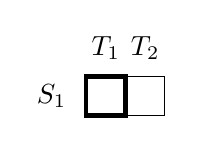
\begin{tikzpicture}[scale=0.5]
  \draw[step=1cm,] (0,0) grid (2,1);
  %\fill[black!20](0,0) rectangle +(1,1);
  \draw[black, ultra thick](0,0) rectangle +(1,1);
\node[anchor=north] at (0.5,2.25) {$T_1$};
\node[anchor=north] at (1.5,2.25) {$T_2$};
\node[anchor=west] at (-1.5,0.5) {$S_1$};
\end{tikzpicture}
& 
\begin{tikzpicture}[scale=0.5]
  \draw[step=1cm,] (0,0) grid (2,1);

(1,0) rectangle +(1,1);
\draw[pattern={north west lines},pattern color=red]
(1,0) rectangle +(1,1);
\draw[pattern={horizontal lines},pattern color=blue](0,0) rectangle (1,1);
\node[anchor=north] at (0.5,2.25) {$T_1$};
\node[anchor=north] at (1.5,2.25) {$T_2$};
\node[anchor=west] at (-1.5,0.5) {$S_1$};
\end{tikzpicture} 
& 
\begin{tikzpicture}[scale=0.5]
  \draw[step=1cm,] (0,0) grid (2,1);
\draw[pattern={north west lines},pattern color=red](0,0) rectangle (1,1);
\draw[pattern={horizontal lines},pattern color=blue](1,0) rectangle +(1,1);
\node[anchor=north] at (0.5,2.25) {$T_1$};
\node[anchor=north] at (1.5,2.25) {$T_2$};
\node[anchor=west] at (-1.5,0.5) {$S_1$};
\end{tikzpicture}\\
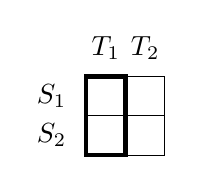
\begin{tikzpicture}[scale=0.5]

%\draw[pattern={north west lines},pattern color=blue](0,0) rectangle +(1,2);
\draw[black, ultra thick](0,0) rectangle +(1,2);
%\draw[pattern={horizontal lines},pattern color=red](1,0) rectangle (2,2);
%\draw[pattern={horizontal lines},pattern color=blue](1,0) rectangle (2,2);
  \draw[step=1cm,] (0,0) grid (2,2);

\node[anchor=north] at (0.5,3.25) {$T_1$};
\node[anchor=north] at (1.5,3.25) {$T_2$};
\node[anchor=west] at (-1.5,1.5) {$S_1$};
\node[anchor=west] at (-1.5,0.5) {$S_2$};
\end{tikzpicture} & \begin{tikzpicture}[scale=0.5]

(0,1) rectangle +(1,1);
\draw[pattern={horizontal lines},pattern color=blue]
(0,1) rectangle +(1,1);
;
\draw[pattern={north west lines},pattern color=red](1,0) rectangle (2,2);
  \draw[step=1cm,] (0,0) grid (2,2);

\node[anchor=north] at (0.5,3.25) {$T_1$};
\node[anchor=north] at (1.5,3.25) {$T_2$};
\node[anchor=west] at (-1.5,1.5) {$S_1$};
\node[anchor=west] at (-1.5,0.5) {$S_2$};
\end{tikzpicture} &
\begin{tikzpicture}[scale=0.5]
(0,0) rectangle +(1,2);
\draw[pattern={north west lines},pattern color=red]
(0,0) rectangle +(1,2);
\draw[pattern={horizontal lines},pattern color=blue](1,1) rectangle +(1,1);
  \draw[step=1cm,] (0,0) grid (2,2);

\node[anchor=north] at (0.5,3.25) {$T_1$};
\node[anchor=north] at (1.5,3.25) {$T_2$};
\node[anchor=west] at (-1.5,1.5) {$S_1$};
\node[anchor=west] at (-1.5,0.5) {$S_2$};
\end{tikzpicture}\\
(a)&(b)&(c)\\

    \end{tabular}
    \end{center}
        \caption{We illustrate the partition for both $\boldsymbol{d}=(1,2)$ and $\boldsymbol{d}=(2,2)$. The set of items $S_1$ can be divided into $T_1$ and $T_2$. If agent $S$ values bundle $T_1 \cap S_1$ (represented with a thick line in (a)) more than $\frac{v_S(S_1)}{2}$ then allocation (b) has the desired properties (the blue bundle for agent $S$ and the red bundle for agent $T$). If this is not the case, then due to the subadditivity, the same holds for agent $S$ and bundle $T_2 \cap S_1$; then (b) has the desired properties.} 
    \label{fig:2agentsRed}
\end{figure}
\end{center}
We also provide a useful restatement of Lemma~\ref{Lemma:2agents} to be used as a reduction tool in the proofs with more agents.
\begin{corollary}
\label{Cor:cut-and-choose}
    Consider a fair division instance of two agents with subadditive valuations and a set of $M$ items, where one agent values $M$ at least $1$, and there exists a partition into two bundles where the other agent values each at least $1/2$. Then, there exists an allocation that guarantees at least $1/2$ value to each agent.
\end{corollary}



\subsection{Three Agents}
\label{sec:3Subadd}
In this section we show that there exists a $1/2$-MMS allocation for the case of three agents. Again, we first show a stronger statement (Lemma~\ref{Lemma:threehalfs}) and obtain the main result as a corollary (Corollary~\ref{cor:3agents}). 

\begin{lemma} [Three agents]
\label{Lemma:threehalfs}
    An $1/2$-MMS$(3,2,2)$ allocation exists for three agents with subadditive valuation functions.
\end{lemma}
\begin{proof}
We denote by $S,T,Q$ the three agents and by $S_j,T_j,Q_j$ their $j$-th MMS bundle, respectively. 

The proof relies on the existence of $(1/2,1)$-MMS$(1,2)$ in the instance with two agents; we show that we can identify a valuable subset $A_T$ (with value at least $1/2$) to allocate to agent $T$, such that we can extend the allocation applying Corollary \ref{Cor:cut-and-choose} for agents $S$ and $Q$ and for the remaining items $M\setminus A_T$. In particular, agent $Q$ will have value at least $1$ for $M\setminus A_T$, while agent $S$ will be able to partition it into two bundles with value at least $1/2$ each. To achieve this we will use two cuts sequentially, first to agent $S$ and then (based on the response of $S$) to agent $T$  (we refer the reader to Figure~\ref{fig:3agents} (a) for an illustration of the proof).
    
{\bf First cut.} Consider the cut $C=T_2$ that we offer to $S$ and let $S_1^*,S_2^* \in \mathcal{X}_{S}^*(C)$ be two bundles in the maximum desired half (by Observation~\ref{obs:Cut_noOfDesiredSets} there exist at least two such bundles). The cut is ``symmetric'' for $T$ in a sense that both $C=T_2$ and $M\setminus C=T_1$ contain the {\em same number of $T$'s MMS bundles}; so it is without loss of generality to assume that $\mathcal{X}^*_S(C)=\mathcal{X}_S(C)$ (in Figure~\ref{fig:3agents} (a) $S_1^* \subseteq S_1,S_2^* \subseteq S_2$ are represented with blue color).

{\bf Second cut.} We next offer $C=Q_1$ to $T$ and let  $T_1^* \in \mathcal{X}_T^*(C)$ be the bundle in the maximum desired half. The cut is ``symmetric'' for $Q$, so again without loss of generality assume that $\mathcal{X}_T^*(C)=\mathcal{X}_T(C)$ (in Figure~\ref{fig:3agents} (b) $T_1^* \subseteq T_1$ is represented with red color).

    
{\bf Apply Corollary \ref{Cor:cut-and-choose}.} Overall, $v_T(T^*_1)\geq 1/2$ and $T^*_1$ will be allocated to $T$. Then, for $M'=M\setminus T^*_1$, it holds that $v_Q(M')\geq v_Q(Q_2) \geq 1$, and $S_1^*,S_2^*\subseteq M'$, for both of which $S$ has value at least $1/2$. So the lemma follows by using Corollary \ref{Cor:cut-and-choose} on $M'$ for agents $Q$ and $S$. (in Figure~\ref{fig:3agents} (c) $S_1^* \subseteq S_1,S_1^* \subseteq S_2$ are represented with blue color and $Q_2$ with green).
\end{proof}
\begin{center}

\begin{figure}
\begin{center}

\begin{tabular}{ccc}

\small{
\begin{tikzpicture}[scale=0.45]
\draw[yslant=0.5,xslant=-1,black, ultra thick](3,3) (5,1) rectangle +(-2,-1);  
\draw[yslant=0.5,black, ultra thick](3,-3) rectangle +(2,3);    \draw[yslant=-0.5,black, ultra thick](3,3) rectangle +(-1,-3); 
\draw[yslant=0.5,xslant=-1,pattern={horizontal lines},pattern color=blue] (5,1) rectangle +(-2,-1);  
\draw[yslant=0.5,pattern={horizontal lines},pattern color=blue](3,-2) rectangle +(2,2);    \draw[yslant=-0.5,pattern={horizontal lines},pattern color=blue](3,3) rectangle +(-1,-2);     

    \draw[yslant=-0.5] (1,0) grid (3,3);
  \draw[yslant=0.5] (3,-3) grid (5,0);
  \draw[yslant=0.5,xslant=-1] (3,0) grid (5,2);
\node[anchor=south west] at (-0.2,1.5,0) {$S_1$};
\node[anchor=south west] at (-0.2,0.5,0) {$S_2$};
\node[anchor=south west] at (-0.2,-0.5,0) {$S_3$};
\node[anchor=north west] at (0.45,3.7,0) {$Q_1$};
\node[anchor=north west] at (1.5,4.3,0) {$Q_2$};
\node[anchor=north west] at (0.5,-0.8,0) {$T_1$};
\node[anchor=north west] at (1.5,-1.3,0) {$T_2$};
\end{tikzpicture}} &
\small{
\begin{tikzpicture}[scale=0.45]
  
    \draw[yslant=0.5,xslant=-1,color=black,ultra thick] (4,2) rectangle +(-1,-2);
    %\fill[yslant=0.5,xslant=-1,color=black!20](4,2) rectangle +(-1,-2); 
    \draw[yslant=0.5,color=black,ultra thick] (3,-3) rectangle +(1,3);
    %\fill[yslant=0.5,color=black!20](3,-3) rectangle +(1,3);

    \draw[yslant=-0.5,color=black,ultra thick](3,3) rectangle +(-2,-3);
    %\fill[yslant=-0.5,color=black!20](3,3) rectangle +(-2,-3);
    
    \draw[yslant=0.5,xslant=-1,pattern={north west lines},pattern color=red](4,2) rectangle +(-1,-1);
\draw[yslant=-0.5,pattern={north west lines},pattern color=red](2,3) rectangle +(-1,-3);
  \draw[yslant=-0.5] (1,0) grid (3,3);
  \draw[yslant=0.5] (3,-3) grid (5,0);
  \draw[yslant=0.5,xslant=-1] (3,0) grid (5,2);
\node[anchor=south west] at (-0.2,1.5,0) {$S_1$};
\node[anchor=south west] at (-0.2,0.5,0) {$S_2$};
\node[anchor=south west] at (-0.2,-0.5,0) {$S_3$};
\node[anchor=north west] at (0.45,3.7,0) {$Q_1$};
\node[anchor=north west] at (1.5,4.3,0) {$Q_2$};
\node[anchor=north west] at (0.5,-0.8,0) {$T_1$};
\node[anchor=north west] at (1.5,-1.3,0) {$T_2$};
\end{tikzpicture}} &
\small{
\begin{tikzpicture}[scale=0.45]
 \draw[yslant=0.5,xslant=-1,pattern={north west lines},pattern color=red](4,2) rectangle +(-1,-1);
\draw[yslant=-0.5,pattern={north west lines},pattern color=red](2,3) rectangle +(-1,-3);
\draw[yslant=0.5,xslant=-1,pattern={crosshatch dots},pattern color=green]  (5,2) rectangle +(-1,-2);
    \draw[yslant=0.5,pattern={crosshatch dots},pattern color=green]  (4,-3) rectangle +(1,3);

    \draw[yslant=0.5,xslant=-1,pattern={horizontal lines},pattern color=blue] (5,1) rectangle +(-2,-1);
    \draw[yslant=0.5,pattern={horizontal lines},pattern color=blue](3,-2) rectangle +(2,2);
    \draw[yslant=-0.5,pattern={horizontal lines},pattern color=blue](3,3) rectangle (2,1);
  \draw[yslant=-0.5] (1,0) grid (3,3);
  \draw[yslant=0.5] (3,-3) grid (5,0);
  \draw[yslant=0.5,xslant=-1] (3,0) grid (5,2);
\node[anchor=south west] at (-0.2,1.5,0) {$S_1$};
\node[anchor=south west] at (-0.2,0.5,0) {$S_2$};
\node[anchor=south west] at (-0.2,-0.5,0) {$S_3$};
\node[anchor=north west] at (0.45,3.7,0) {$Q_1$};
\node[anchor=north west] at (1.5,4.3,0) {$Q_2$};
\node[anchor=north west] at (0.5,-0.8,0) {$T_1$};
\node[anchor=north west] at (1.5,-1.3,0) {$T_2$};
\end{tikzpicture}}\\
(a) & (b) & (c) \\
$S_1^*,S_2^* \in \mathcal{X}_S^*(T_2)$ &  $T_1^* \in \mathcal{X}^*_T(Q_1)$ & Apply Corollary \ref{Cor:cut-and-choose}\\
\end{tabular}
    
\end{center}
\caption{We use blue, red, and green to denote the bundles from which we will allocate to agents $S,T$ and $Q$, respectively. The thickened lines illustrate the first and second cuts, while (c) demonstrates the application of Corollary 2.
}
\label{fig:3agents}
\end{figure} 
\end{center}
As a corollary of Lemma~\ref{Lemma:threehalfs}, a $1/2$-MMS allocation always exists for three agents (by Observation~\ref{obs:simpleReduction}); this bound is also tight \cite{GhodsiHSSY22}. 
\begin{corollary}
\label{cor:3agents}
    A $1/2$-MMS allocation exists for three agents with subadditive valuation functions. 
\end{corollary}


\subsection{Four Agents}
In this section we show the existence of $1/2$-MMS allocation for the case of four agents, our main technical result. We are also able to show a stronger statement (Lemma~\ref{Lemma:4agents}) and obtain the main result as a corollary (Corollary~\ref{cor:4agents}). 

\label{sec:4Subadd}

\begin{lemma} [Four agents]
\label{Lemma:4agents}
    A $1/2$-MMS$(3,3,4,4)$ allocation exists for four agents with subadditive valuation functions.
\end{lemma}
\begin{proof}
    We denote by $S,T,Q,R$ the four agents and by $S_j,T_j,Q_j,R_j$ their $j$-th MMS bundle, respectively. 
    
    We progressively identify four candidate allocations in total, and we show that one of those should be a $1/2$-MMS$(3,3,4,4)$ allocation. 

    In a nutshell, the protocol works as follows. By offering carefully chosen cuts to agents $S,T,Q$ we are able to find partial allocations for two of those agents (in the first round these are $S$ and $T$), that have high enough value (higher than $1/2$), in a way that always preserves one MMS bundle of agent $R$ {\em intact}, let it be $R_4$. If the third agent (this is $Q$ in the first round) values higher than $1/2$ two of her bundles (on the remaining items) then we can apply Corollary~\ref{Cor:cut-and-choose} on $Q$ and $R$ and for the remaining items, and we can claim a $1/2$-MMS$(3,3,4,4)$ allocation. If this is not the case, then the third agent must value at least two of the intersections of her bundles with the partial allocation of the other two agents with value higher than $1/2$. In the next round we will tentatively allocate to the third agent one of these sets. We will also keep one of the other two agents and offer her a subset of high value {\em from a different bundle} (the notion of maximum desired half is useful to achieve this last property). We proceed in a similar manner by querying the remaining agent investigating again whether Corollary~\ref{Cor:cut-and-choose} can be employed. The key is that in every round that the third agent does not satisfy the conditions of Corollary~\ref{Cor:cut-and-choose} we are able to build a more structured partial allocation, which in the final step provides an allocation of $M\setminus R_4$ to agents $S,T$ and $Q$, that they value by at least $1/2$. Then $R_4$ can be allocated to agent $R$ and the allocation is $1/2$-MMS$(3,3,4,4)$.
    
\begin{center}

\begin{figure}[t]
\begin{center}

    \begin{tabular}{cc}
\small{
\begin{tikzpicture}[scale=0.425]
\draw[yslant=0.5,ultra thick, black](4,-3) rectangle +(4,1);     
\draw[yslant=-0.5,ultra thick, black](4,2) rectangle +(-3,-1); 
\draw[yslant=-0.5,pattern={north west lines},pattern color=red](4,3) rectangle +(-1,-1);
\draw[yslant=-0.5,pattern={north west lines},pattern color=red](4,1) rectangle +(-1,-1);
\draw[yslant=0.5,xslant=-1,pattern={north west lines},pattern color=red](7,0) rectangle +(-4,-1); 
\draw[yslant=0.5,pattern={north west lines},pattern color=red](4,-2) rectangle +(4,1);   
\draw[yslant=0.5,pattern={north west lines},pattern color=red](4,-4) rectangle +(4,1);   
%\draw[yslant=0.5,xslant=-1,pattern={horizontal lines},pattern color=blue](7,2) rectangle +(-4,-3);  
\draw[yslant=0.5,pattern={horizontal lines},pattern color=blue](4,-3) rectangle +(4,1);     
\draw[yslant=-0.5,pattern={horizontal lines},pattern color=blue](4,2) rectangle +(-3,-1);     
  \draw[yslant=-0.5] (1,0) grid (4,3);
  \draw[yslant=0.5] (4,-4) grid (8,-1);
  \draw[yslant=0.5,xslant=-1] (3,-1) grid (7,2);
\node[anchor=south west] at (-0.25,1.5,0) {$S_1$};
\node[anchor=south west] at (-0.25,0.5,0) {$S_2$};
\node[anchor=south west] at (-0.25,-0.5,0) {$S_3$};
\node[anchor=north west] at (0.5,3.8,0) {$Q_1$};
\node[anchor=north west] at (1.5,4.3,0) {$Q_2$};
\node[anchor=north west] at (2.5,4.8,0) {$Q_3$};
\node[anchor=north west] at (3.5,5.3,0) {$Q_4$};
\node[anchor=north west] at (0.4,-0.8,0) {$T_3$};
\node[anchor=north west] at (1.4,-1.3,0) {$T_2$};
\node[anchor=north west] at (2.4,-1.8,0) {$T_1$};
\node[anchor=north] at (7,5,0) {$R_1$};
\end{tikzpicture}}
&
\small{
\begin{tikzpicture}[scale=0.425]
\draw[yslant=0.5,ultra thick, black](4,-3) rectangle +(4,1);     
\draw[yslant=-0.5,ultra thick, black](4,2) rectangle +(-3,-1); 
\draw[yslant=-0.5,pattern={north west lines},pattern color=red](4,3) rectangle +(-1,-1);
\draw[yslant=-0.5,pattern={north west lines},pattern color=red](4,1) rectangle +(-1,-1);
\draw[yslant=0.5,xslant=-1,pattern={north west lines},pattern color=red](7,0) rectangle +(-4,-1); 
\draw[yslant=0.5,pattern={north west lines},pattern color=red](4,-2) rectangle +(4,1);   
\draw[yslant=0.5,pattern={north west lines},pattern color=red](4,-4) rectangle +(4,1);   
%\draw[yslant=0.5,xslant=-1,pattern={horizontal lines},pattern color=blue](7,2) rectangle +(-4,-3);  
\draw[yslant=0.5,pattern={horizontal lines},pattern color=blue](4,-3) rectangle +(4,1);     
\draw[yslant=-0.5,pattern={horizontal lines},pattern color=blue](4,2) rectangle +(-3,-1);      
  \draw[yslant=-0.5] (1,0) grid (4,3);
  \draw[yslant=0.5] (4,-4) grid (8,-1);
  \draw[yslant=0.5,xslant=-1] (3,-1) grid (7,2);
\node[anchor=south west] at (-0.25,1.5,0) {$S_1$};
\node[anchor=south west] at (-0.25,0.5,0) {$S_2$};
\node[anchor=south west] at (-0.25,-0.5,0) {$S_3$};
\node[anchor=north west] at (0.5,3.8,0) {$Q_1$};
\node[anchor=north west] at (1.5,4.3,0) {$Q_2$};
\node[anchor=north west] at (2.5,4.8,0) {$Q_3$};
\node[anchor=north west] at (3.5,5.3,0) {$Q_4$};
\node[anchor=north west] at (0.4,-0.8,0) {$T_3$};
\node[anchor=north west] at (1.4,-1.3,0) {$T_2$};
\node[anchor=north west] at (2.4,-1.8,0) {$T_1$};
\node[anchor=north] at (7,5,0) {$R_2$};
\end{tikzpicture}}\\
\small{
\begin{tikzpicture}[scale=0.425]
\draw[yslant=-0.5,pattern={north west lines},pattern color=red](4,3) rectangle +(-1,-3);
\draw[yslant=0.5,xslant=-1,pattern={north west lines},pattern color=red](7,0) rectangle +(-4,-1); 
\draw[yslant=0.5,pattern={north west lines},pattern color=red](4,-4) rectangle +(4,3);    
  \draw[yslant=-0.5] (1,0) grid (4,3);
  \draw[yslant=0.5] (4,-4) grid (8,-1);
  \draw[yslant=0.5,xslant=-1] (3,-1) grid (7,2);
\node[anchor=south west] at (-0.25,1.5,0) {$S_1$};
\node[anchor=south west] at (-0.25,0.5,0) {$S_2$};
\node[anchor=south west] at (-0.25,-0.5,0) {$S_3$};
\node[anchor=north west] at (0.5,3.8,0) {$Q_1$};
\node[anchor=north west] at (1.5,4.3,0) {$Q_2$};
\node[anchor=north west] at (2.5,4.8,0) {$Q_3$};
\node[anchor=north west] at (3.5,5.3,0) {$Q_4$};
\node[anchor=north west] at (0.4,-0.8,0) {$T_3$};
\node[anchor=north west] at (1.4,-1.3,0) {$T_2$};
\node[anchor=north west] at (2.4,-1.8,0) {$T_1$};
\node[anchor=north] at (7,5,0) {$R_3$};
\end{tikzpicture}}
&

\small{
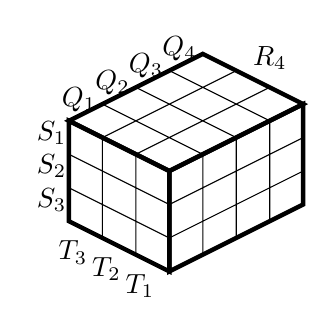
\begin{tikzpicture}[scale=0.425]
\draw[yslant=0.5,ultra thick, black](4,-4) rectangle +(4,3);     
\draw[yslant=-0.5,ultra thick, black](4,3) rectangle +(-3,-3); 
\draw[yslant=0.5,xslant=-1,ultra thick, black](7,2) rectangle +(-4,-3);    
  \draw[yslant=-0.5] (1,0) grid (4,3);
  \draw[yslant=0.5] (4,-4) grid (8,-1);
  \draw[yslant=0.5,xslant=-1] (3,-1) grid (7,2);
\node[anchor=south west] at (-0.25,1.5,0) {$S_1$};
\node[anchor=south west] at (-0.25,0.5,0) {$S_2$};
\node[anchor=south west] at (-0.25,-0.5,0) {$S_3$};
\node[anchor=north west] at (0.5,3.8,0) {$Q_1$};
\node[anchor=north west] at (1.5,4.3,0) {$Q_2$};
\node[anchor=north west] at (2.5,4.8,0) {$Q_3$};
\node[anchor=north west] at (3.5,5.3,0) {$Q_4$};
\node[anchor=north west] at (0.4,-0.8,0) {$T_3$};
\node[anchor=north west] at (1.4,-1.3,0) {$T_2$};
\node[anchor=north west] at (2.4,-1.8,0) {$T_1$};
\node[anchor=north] at (7,5,0) {$R_4$};
\end{tikzpicture}}\\
\end{tabular}
    
\end{center}
\caption{The first candidate allocation $A=(S_2^*,T_1^*)$ for four agents and $\boldsymbol{d}=(3,3,4,4)$. We use blue to denote $S_2^* \subseteq S_2$ and red to denote $T_1^* \subseteq T_1$. We use a thick line to illustrate the cut $C=\{S^*_2 \cup R_4\}$. The allocation is valid and none of the bundles intersects with $R_4$. The cuts are symmetric, i.e. if we had $\mathcal{X}_S^*(C) =\mathcal{X}_S^*(M\setminus C)$ for cut $C=\{R_1 \cup R_2\}$ or/and $\mathcal{X}_T^*(C)=\mathcal{X}_T(C)$ for the corresponding cut $C$, we could construct the same allocation by renaming the bundles.}
\label{fig:4agents1}
\end{figure}
\end{center}



    
  
    
    \noindent{\bf Building the first candidate allocation}. We first consider agent $S$ (an agent with $3$ MMS bundles) and cut her MMS bundles by offering the cut $C=R_1 \cup R_2$. By Observation~\ref{obs:Cut_noOfDesiredSets} there are at least two bundles in the set $\mathcal{X}_{S}^*(C)$; let those be $S_1^*,S_2^* \in \mathcal{X}_{S}^*(C)$. We note that $S_1^*,S_2^*$ intersect with exactly two MMS bundles of $R$, so w.l.o.g. assume that those are $R_1,R_2$, i.e., assume that $\mathcal{X}_{S}^*(C)=\mathcal{X}_{S}(C)$. Therefore
     \begin{equation}
        \label{eq:4agentsCond0}
        S_j^*\cap R_3 = \emptyset \mbox{ and } S_j^*\cap R_4 = \emptyset, \mbox{ for } j \in \{1,2\}\,.
    \end{equation}
    

    Next, we offer a cut to agent $T$ in a way that a) ensures that a {\em whole} MMS bundle of agent $R$ remains intact and b) one of $S_1^*, S_2^*$ does not intersect with the Maximum Desired Half of $T$. A cut that serves this purpose is $C=S_2^* \cup R_4$. Now each of the sets $C$ and $M\setminus C$ intersects with exactly one of $S^*_1, S^*_2$ and with exactly one of $R_3, R_4$ which are the remaining whole bundles of $R$. W.l.o.g. assume that $\mathcal{X}_{T}^*(C)=\mathcal{X}_{T}(M \setminus C)$.\footnote{Even if it is w.l.o.g., we consider $\mathcal{X}_{T}^*(C)=\mathcal{X}_{T}(M \setminus C)$ that includes $S_3$ to avoid any confusion of the steps needed, because the case of $\mathcal{X}_{T}^*(C)=\mathcal{X}_{T}(C)$ is simpler and can be handled the same way.} 
    By Observation~\ref{obs:Cut_noOfDesiredSets} there are at least two bundles in the set $\mathcal{X}_{T}^*(C)$, let those be $T_1^*,T_2^* \in \mathcal{X}_{T}^*(C)$. Then, it holds that 
    \begin{equation}
    \label{eq:4agentsCond1}
        T_j^*\cap R_4 = \emptyset \mbox{ and } T_j^*\cap S_2^* = \emptyset, \mbox{ for } j \in \{1,2\}\,.
    \end{equation}
    
    {\bf First candidate allocation.} Consider the following partial allocation for $S$ and $T$: $A= (S^*_2,T^*_1)$ (see Figure \ref{fig:4agents1} for an illustration). By construction, both $S$ and $T$ value their allocated bundles by at least $1/2$. If there exist at least two MMS bundles of $Q$ that she values with at least $1/2$ {\em after the removal of $S^*_2\cup T^*_1$}, then the conditions of Corollary~\ref{Cor:cut-and-choose} are satisfied for $Q$ and $R$ for the remaining items (recall that $R$ values the remaining items by at least $1$ since they contain $R_4$). Hence by  employing Corollary~\ref{Cor:cut-and-choose} we can find an allocation of $M\setminus (S^*_2\cup T^*_1)$ to $Q$ and $R$ where they both value their bundles with at least $1/2$, and we are done.   
        
    So, suppose that this is not the case. Then there must be at least three MMS bundles of $Q$, let them be $Q_1,Q_2,Q_3$, such that $v_Q(Q_j\cap(S^*_2\cup T^*_1))\geq 1/2$ for $j\in\{1, 2, 3\}$. In other words, if we consider the cut $C=S^*_2\cup T^*_1$ for agent $Q$, then it is guaranteed that $Q_1^*,Q^*_2,Q^*_3 \in \mathcal{X}_{Q}(C)$. Since $Q_j^*\subseteq S^*_2\cup T^*_1$, for all $j \in \{1,2,3\}$ and also by \eqref{eq:4agentsCond0} and \eqref{eq:4agentsCond1} we conclude that
    \begin{equation}
        \label{eq:4agentsCond2}
        Q_j^* \cap T^*_2 = \emptyset \mbox{ and } Q_j^* \cap R_4= \emptyset , \mbox{ for } j \in \{1,2,3\}\,.
    \end{equation}


    \begin{figure}[h] 
\begin{center}
    \begin{tabular}{cc}
\small{
\begin{tikzpicture}[scale=0.425]
\draw[yslant=-0.5,ultra thick, black](4,3) rectangle +(-1,-3);
\draw[yslant=0.5,xslant=-1,ultra thick, black](7,0) rectangle +(-4,-1); 
\draw[yslant=0.5,ultra thick, black](4,-4) rectangle +(4,3);   
       
\draw[yslant=-0.5,ultra thick, black](3,2) rectangle +(-2,-1);
\draw[yslant=-0.5,ultra thick, white](3,2) rectangle +(0,-1);
\draw[yslant=0.5,pattern={crosshatch dots},pattern color=green] (4,-4) rectangle +(1,3);
\draw[yslant=-0.5,pattern={crosshatch dots},pattern color=green](4,3) rectangle +(-1,-3);
\draw[yslant=-0.5,pattern={crosshatch dots},pattern color=green](3,2) rectangle +(-2,-1);
\draw[yslant=-0.5,pattern={north west lines},pattern color=red](3,3) rectangle +(-1,-1);
\draw[yslant=-0.5,pattern={north west lines},pattern color=red](3,1) rectangle +(-1,-1);
\draw[yslant=0.5,xslant=-1,pattern={north west lines},pattern color=red](7,1) rectangle +(-4,-1); 
\draw[yslant=0.5,xslant=-1,pattern={crosshatch dots},pattern color=green](4,0) rectangle +(-1,-1);     
  \draw[yslant=-0.5] (1,0) grid (4,3);
  \draw[yslant=0.5] (4,-4) grid (8,-1);
  \draw[yslant=0.5,xslant=-1] (3,-1) grid (7,2);
\node[anchor=south west] at (-0.25,1.5,0) {$S_1$};
\node[anchor=south west] at (-0.25,0.5,0) {$S_2$};
\node[anchor=south west] at (-0.25,-0.5,0) {$S_3$};
\node[anchor=north west] at (0.5,3.8,0) {$Q_1$};
\node[anchor=north west] at (1.5,4.3,0) {$Q_2$};
\node[anchor=north west] at (2.5,4.8,0) {$Q_3$};
\node[anchor=north west] at (3.5,5.3,0) {$Q_4$};
\node[anchor=north west] at (0.4,-0.8,0) {$T_3$};
\node[anchor=north west] at (1.4,-1.3,0) {$T_2$};
\node[anchor=north west] at (2.4,-1.8,0) {$T_1$};
\node[anchor=north] at (7,5,0) {$R_1$};
\end{tikzpicture}}
&
\small{
\begin{tikzpicture}[scale=0.425]
\draw[yslant=-0.5,ultra thick, black](4,3) rectangle +(-1,-3);
\draw[yslant=0.5,xslant=-1,ultra thick, black](7,0) rectangle +(-4,-1); 
\draw[yslant=0.5,ultra thick, black](4,-4) rectangle +(4,3);   
       
\draw[yslant=-0.5,ultra thick, black](3,2) rectangle +(-2,-1);
\draw[yslant=-0.5,ultra thick, white](3,2) rectangle +(0,-1);
\draw[yslant=0.5,pattern={crosshatch dots},pattern color=green] (4,-4) rectangle +(1,3);
\draw[yslant=-0.5,pattern={crosshatch dots},pattern color=green](4,3) rectangle +(-1,-3);
\draw[yslant=-0.5,pattern={crosshatch dots},pattern color=green](3,2) rectangle +(-2,-1);
\draw[yslant=-0.5,pattern={north west lines},pattern color=red](3,3) rectangle +(-1,-1);
\draw[yslant=-0.5,pattern={north west lines},pattern color=red](3,1) rectangle +(-1,-1);
\draw[yslant=0.5,xslant=-1,pattern={north west lines},pattern color=red](7,1) rectangle +(-4,-1); 
\draw[yslant=0.5,xslant=-1,pattern={crosshatch dots},pattern color=green](4,0) rectangle +(-1,-1);    
  \draw[yslant=-0.5] (1,0) grid (4,3);
  \draw[yslant=0.5] (4,-4) grid (8,-1);
  \draw[yslant=0.5,xslant=-1] (3,-1) grid (7,2);
\node[anchor=south west] at (-0.25,1.5,0) {$S_1$};
\node[anchor=south west] at (-0.25,0.5,0) {$S_2$};
\node[anchor=south west] at (-0.25,-0.5,0) {$S_3$};
\node[anchor=north west] at (0.5,3.8,0) {$Q_1$};
\node[anchor=north west] at (1.5,4.3,0) {$Q_2$};
\node[anchor=north west] at (2.5,4.8,0) {$Q_3$};
\node[anchor=north west] at (3.5,5.3,0) {$Q_4$};
\node[anchor=north west] at (0.4,-0.8,0) {$T_3$};
\node[anchor=north west] at (1.4,-1.3,0) {$T_2$};
\node[anchor=north west] at (2.4,-1.8,0) {$T_1$};
\node[anchor=north] at (7,5,0) {$R_2$};
\end{tikzpicture}}\\
\small{
\begin{tikzpicture}[scale=0.425]
\draw[yslant=-0.5,ultra thick, black](4,3) rectangle +(-1,-3);
\draw[yslant=0.5,xslant=-1,ultra thick, black](7,0) rectangle +(-4,-1); 
\draw[yslant=0.5,ultra thick, black](4,-4) rectangle +(4,3);   
       
\draw[yslant=-0.5,pattern={north west lines},pattern color=red](3,3) rectangle +(-1,-3);
\draw[yslant=0.5,xslant=-1,pattern={north west lines},pattern color=red](7,1) rectangle +(-4,-1); 
\draw[yslant=-0.5,pattern={crosshatch dots},pattern color=green](4,3) rectangle +(-1,-3);
\draw[yslant=0.5,xslant=-1,pattern={crosshatch dots},pattern color=green](4,0) rectangle +(-1,-1); 
\draw[yslant=0.5,pattern={crosshatch dots},pattern color=green](4,-4) rectangle +(1,3);    
  \draw[yslant=-0.5] (1,0) grid (4,3);
  \draw[yslant=0.5] (4,-4) grid (8,-1);
  \draw[yslant=0.5,xslant=-1] (3,-1) grid (7,2);
\node[anchor=south west] at (-0.25,1.5,0) {$S_1$};
\node[anchor=south west] at (-0.25,0.5,0) {$S_2$};
\node[anchor=south west] at (-0.25,-0.5,0) {$S_3$};
\node[anchor=north west] at (0.5,3.8,0) {$Q_1$};
\node[anchor=north west] at (1.5,4.3,0) {$Q_2$};
\node[anchor=north west] at (2.5,4.8,0) {$Q_3$};
\node[anchor=north west] at (3.5,5.3,0) {$Q_4$};
\node[anchor=north west] at (0.4,-0.8,0) {$T_3$};
\node[anchor=north west] at (1.4,-1.3,0) {$T_2$};
\node[anchor=north west] at (2.4,-1.8,0) {$T_1$};
\node[anchor=north] at (7,5,0) {$R_3$};
\end{tikzpicture}}
&

\small{
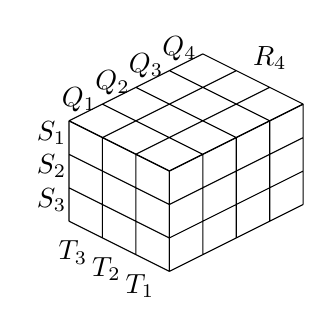
\begin{tikzpicture}[scale=0.425]

    
  \draw[yslant=-0.5] (1,0) grid (4,3);
  \draw[yslant=0.5] (4,-4) grid (8,-1);
  \draw[yslant=0.5,xslant=-1] (3,-1) grid (7,2);
\node[anchor=south west] at (-0.25,1.5,0) {$S_1$};
\node[anchor=south west] at (-0.25,0.5,0) {$S_2$};
\node[anchor=south west] at (-0.25,-0.5,0) {$S_3$};
\node[anchor=north west] at (0.5,3.8,0) {$Q_1$};
\node[anchor=north west] at (1.5,4.3,0) {$Q_2$};
\node[anchor=north west] at (2.5,4.8,0) {$Q_3$};
\node[anchor=north west] at (3.5,5.3,0) {$Q_4$};
\node[anchor=north west] at (0.4,-0.8,0) {$T_3$};
\node[anchor=north west] at (1.4,-1.3,0) {$T_2$};
\node[anchor=north west] at (2.4,-1.8,0) {$T_1$};
\node[anchor=north] at (7,5,0) {$R_4$};
\end{tikzpicture}}\\
\end{tabular}
    
\end{center}
\caption{The second candidate allocation $A'=(T_2^*,Q_1^*)$. We use red for bundle $T_2^* \subseteq T_2$ and green for $Q_1^*\subseteq Q_1$. The cut $C=\{T_1^* \cup S_2^*\}$ is shown with a thick line. We try to apply Corollary \ref{cor:2agents} for agents $S$ and $R$ and the set of items $M \setminus (T_2^*\cup Q_1^*)$. We could construct the same allocation for any $3$ bundles $Q_i^*$ by renaming the bundles.}
\label{fig:4agents2}
\end{figure}

    {\bf Second candidate allocation.} Next, we consider the partial allocation $A'= (T^*_2,Q^*_1)$ for agents $T$ and $Q$ which by (\ref{eq:4agentsCond2}) is valid and both $v_T(T^*_2), v_Q(Q_1^*)$ are higher than $1/2$ (see Figure \ref{fig:4agents2} for an illustration). If there exist at least two MMS bundles of $S$, that she values with at least $1/2$ {\em after the removal of $T^*_2 \cup Q^*_1$}, then by employing Corollary \ref{Cor:cut-and-choose} we can find an allocation of $M\setminus (T^*_2\cup Q^*_1)$ to $S$ and $R$ where they both value their bundles with at least $1/2$, and we are done.
    
    
    Otherwise, it should be that for the cut $C=T^*_2 \cup Q^*_1$  there are two sets\footnote{We note that it is not necessarily the case that $S'_1\subseteq S_1$ or $S'_2\subseteq S_2$ although this is how it is depicted in the figures for the sake of exposition.} $S_1',S_2' \in \mathcal{X}_{S}(C)$. 
    Since for any $j \in \{1,2\}$, $S_j'\subseteq T^*_2 \cup Q^*_1$, by \eqref{eq:4agentsCond1} and \eqref{eq:4agentsCond2} we conclude
    \begin{equation}
        \label{eq:4agentsCond3}
        S_j' \cap Q^*_2 = \emptyset, S_j' \cap Q^*_3 = \emptyset \mbox{ and } S_j' \cap R_4 = \emptyset, \mbox{ for } j \in \{1,2\}\,.
    \end{equation}
    
    
    {\bf Third candidate allocation.} Consider now the partial allocation $A''= (S'_1,Q^*_2)$ for $S$ and $Q$, which is valid (due to (\ref{eq:4agentsCond3})) and both agents value their allocated bundles by at least $1/2$ (see Figure \ref{fig:4agents3} for an illustration).
    Again, if there exist at least two MMS bundles of $T$, that she values with at least $1/2$ after the removal of $S'_1\cup Q^*_2$, by using Corollary \ref{Cor:cut-and-choose} on $T$ and $R$, we are done (similarly as in the previous cases). 
    
 
  

\begin{figure}[H]
\begin{center}

    \begin{tabular}{cc}
\small{
\begin{tikzpicture}[scale=0.425]
      
 
\draw[yslant=0.5,ultra thick, black] (4,-4) rectangle +(1,3);
\draw[yslant=-0.5,ultra thick, black](4,3) rectangle +(-2,-3);
\draw[yslant=-0.5,ultra thick, black](2,2) rectangle +(-1,-1);
\draw[yslant=-0.5,ultra thick, white](3,1) rectangle +(-1,1);
\draw[yslant=0.5,xslant=-1,ultra thick, black](7,1) rectangle +(-4,-1); 
\draw[yslant=0.5,xslant=-1,ultra thick, black](4,0) rectangle +(-1,-1); 
\draw[yslant=0.5,xslant=-1,ultra thick, white](3,0) rectangle +(1,0); 

\draw[yslant=0.5,pattern={crosshatch dots},pattern color=green] (5,-4) rectangle +(1,3);
\draw[yslant=0.5,xslant=-1,pattern={crosshatch dots},pattern color=green](5,0) rectangle +(-1,-1); 
\draw[yslant=0.5,pattern={horizontal lines},pattern color=blue](4,-2) rectangle +(1,1);    
\draw[yslant=0.5,xslant=-1,pattern={horizontal lines},pattern color=blue](7,1) rectangle +(-4,-1);
\draw[yslant=0.5,xslant=-1,pattern={horizontal lines},pattern color=blue](4,0) rectangle +(-1,-1);
%\draw[yslant=-0.5,pattern={horizontal lines},pattern color=blue](4,2) rectangle +(-3,-1);     
\draw[yslant=-0.5,pattern={horizontal lines},pattern color=blue](4,3) rectangle +(-2,-1);    
  \draw[yslant=-0.5] (1,0) grid (4,3);
  \draw[yslant=0.5] (4,-4) grid (8,-1);
  \draw[yslant=0.5,xslant=-1] (3,-1) grid (7,2);
\node[anchor=south west] at (-0.25,1.5,0) {$S_1$};
\node[anchor=south west] at (-0.25,0.5,0) {$S_2$};
\node[anchor=south west] at (-0.25,-0.5,0) {$S_3$};
\node[anchor=north west] at (0.5,3.8,0) {$Q_1$};
\node[anchor=north west] at (1.5,4.3,0) {$Q_2$};
\node[anchor=north west] at (2.5,4.8,0) {$Q_3$};
\node[anchor=north west] at (3.5,5.3,0) {$Q_4$};
\node[anchor=north west] at (0.4,-0.8,0) {$T_3$};
\node[anchor=north west] at (1.4,-1.3,0) {$T_2$};
\node[anchor=north west] at (2.4,-1.8,0) {$T_1$};
\node[anchor=north] at (7,5,0) {$R_1$};
\end{tikzpicture}}
&
\small{
\begin{tikzpicture}[scale=0.425]

\draw[yslant=0.5,ultra thick, black] (4,-4) rectangle +(1,3);
\draw[yslant=-0.5,ultra thick, black](4,3) rectangle +(-2,-3);
\draw[yslant=-0.5,ultra thick, black](2,2) rectangle +(-1,-1);
\draw[yslant=-0.5,ultra thick, white](3,1) rectangle +(-1,1);
\draw[yslant=0.5,xslant=-1,ultra thick, black](7,1) rectangle +(-4,-1); 
\draw[yslant=0.5,xslant=-1,ultra thick, black](4,0) rectangle +(-1,-1); 
\draw[yslant=0.5,xslant=-1,ultra thick, white](3,0) rectangle +(1,0); 

\draw[yslant=0.5,pattern={crosshatch dots},pattern color=green] (5,-4) rectangle +(1,3);

\draw[yslant=0.5,xslant=-1,pattern={crosshatch dots},pattern color=green](5,0) rectangle +(-1,-1); 
\draw[yslant=0.5,pattern={horizontal lines},pattern color=blue](4,-2) rectangle +(1,1);    
\draw[yslant=0.5,xslant=-1,pattern={horizontal lines},pattern color=blue](7,1) rectangle +(-4,-1);
\draw[yslant=0.5,xslant=-1,pattern={horizontal lines},pattern color=blue](4,0) rectangle +(-1,-1);
%\draw[yslant=-0.5,pattern={horizontal lines},pattern color=blue](4,2) rectangle +(-3,-1);     
\draw[yslant=-0.5,pattern={horizontal lines},pattern color=blue](4,3) rectangle +(-2,-1);  
  \draw[yslant=-0.5] (1,0) grid (4,3);
  \draw[yslant=0.5] (4,-4) grid (8,-1);
  \draw[yslant=0.5,xslant=-1] (3,-1) grid (7,2);
\node[anchor=south west] at (-0.25,1.5,0) {$S_1$};
\node[anchor=south west] at (-0.25,0.5,0) {$S_2$};
\node[anchor=south west] at (-0.25,-0.5,0) {$S_3$};
\node[anchor=north west] at (0.5,3.8,0) {$Q_1$};
\node[anchor=north west] at (1.5,4.3,0) {$Q_2$};
\node[anchor=north west] at (2.5,4.8,0) {$Q_3$};
\node[anchor=north west] at (3.5,5.3,0) {$Q_4$};
\node[anchor=north west] at (0.4,-0.8,0) {$T_3$};
\node[anchor=north west] at (1.4,-1.3,0) {$T_2$};
\node[anchor=north west] at (2.4,-1.8,0) {$T_1$};
\node[anchor=north] at (7,5,0) {$R_2$};
\end{tikzpicture}}\\
\small{
\begin{tikzpicture}[scale=0.425]
\draw[yslant=0.5,ultra thick, black] (4,-4) rectangle +(1,3);
\draw[yslant=-0.5,ultra thick, black](4,3) rectangle +(-2,-3);
\draw[yslant=0.5,xslant=-1,ultra thick, black](7,1) rectangle +(-4,-1); 
\draw[yslant=0.5,xslant=-1,ultra thick, black](4,0) rectangle +(-1,-1); 
\draw[yslant=0.5,xslant=-1,ultra thick, white](3,0) rectangle +(1,0); 

\draw[yslant=0.5,pattern={crosshatch dots},pattern color=green] (5,-4) rectangle +(1,3);

\draw[yslant=0.5,xslant=-1,pattern={crosshatch dots},pattern color=green](5,0) rectangle +(-1,-1); 
\draw[yslant=0.5,pattern={horizontal lines},pattern color=blue](4,-2) rectangle +(1,1);    
\draw[yslant=0.5,xslant=-1,pattern={horizontal lines},pattern color=blue](7,1) rectangle +(-4,-1);
\draw[yslant=0.5,xslant=-1,pattern={horizontal lines},pattern color=blue](4,0) rectangle +(-1,-1);
%\draw[yslant=-0.5,pattern={horizontal lines},pattern color=blue](4,2) rectangle +(-3,-1);     
\draw[yslant=-0.5,pattern={horizontal lines},pattern color=blue](4,3) rectangle +(-2,-1);
  \draw[yslant=-0.5] (1,0) grid (4,3);
  \draw[yslant=0.5] (4,-4) grid (8,-1);
  \draw[yslant=0.5,xslant=-1] (3,-1) grid (7,2);
\node[anchor=south west] at (-0.25,1.5,0) {$S_1$};
\node[anchor=south west] at (-0.25,0.5,0) {$S_2$};
\node[anchor=south west] at (-0.25,-0.5,0) {$S_3$};
\node[anchor=north west] at (0.5,3.8,0) {$Q_1$};
\node[anchor=north west] at (1.5,4.3,0) {$Q_2$};
\node[anchor=north west] at (2.5,4.8,0) {$Q_3$};
\node[anchor=north west] at (3.5,5.3,0) {$Q_4$};
\node[anchor=north west] at (0.4,-0.8,0) {$T_3$};
\node[anchor=north west] at (1.4,-1.3,0) {$T_2$};
\node[anchor=north west] at (2.4,-1.8,0) {$T_1$};
\node[anchor=north] at (7,5,0) {$R_3$};
\end{tikzpicture}}
&

\small{
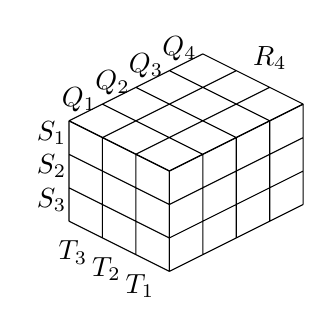
\begin{tikzpicture}[scale=0.425]

    
  \draw[yslant=-0.5] (1,0) grid (4,3);
  \draw[yslant=0.5] (4,-4) grid (8,-1);
  \draw[yslant=0.5,xslant=-1] (3,-1) grid (7,2);
\node[anchor=south west] at (-0.25,1.5,0) {$S_1$};
\node[anchor=south west] at (-0.25,0.5,0) {$S_2$};
\node[anchor=south west] at (-0.25,-0.5,0) {$S_3$};
\node[anchor=north west] at (0.5,3.8,0) {$Q_1$};
\node[anchor=north west] at (1.5,4.3,0) {$Q_2$};
\node[anchor=north west] at (2.5,4.8,0) {$Q_3$};
\node[anchor=north west] at (3.5,5.3,0) {$Q_4$};
\node[anchor=north west] at (0.4,-0.8,0) {$T_3$};
\node[anchor=north west] at (1.4,-1.3,0) {$T_2$};
\node[anchor=north west] at (2.4,-1.8,0) {$T_1$};
\node[anchor=north] at (7,5,0) {$R_4$};
\end{tikzpicture}}\\
\end{tabular}
    
\end{center}

\caption{The third candidate allocation $A''=(S_1',Q_2^*)$. We use blue for bundle $S_1'  \subseteq S_1$ and green color for $Q_2^*\subseteq Q_2$. The cut $C=\{T_2^* \cup Q_1^*\}$ is shown with a thick line. Note that the allocation is valid and none of the bundles intersects with $R_4$. We try to apply Corollary \ref{cor:2agents} for agents $T$ and $R$ and the set of items $M \setminus (T_2^*\cup Q_1^*)$. We could construct a similar allocation for any bundle $S_i'$ and bundle $Q_j$ by renaming the bundles such that $S_i' \cap Q_j^* = \emptyset$ and $S_i' \cap R_4 = \emptyset$.}
\label{fig:4agents3}
\end{figure}


   Otherwise, it should be that for the cut $C=S'_1\cup Q^*_2$ there exist two sets $T_1',T_2' \in \mathcal{X}_{T}(C)$. 
    Since for any $j \in \{1,2\}$, $T_j'\subseteq S'_1\cup Q^*_2$, by \eqref{eq:4agentsCond2} and \eqref{eq:4agentsCond3} it holds that 
      \begin{equation}
        \label{eq:4agentsCond4}
        T_j' \cap Q^*_3 = \emptyset, T_j' \cap S'_2 = \emptyset \mbox{ and } T_j' \cap R_4 = \emptyset, \mbox{ for } j \in \{1,2\}\,.
    \end{equation}
    



\begin{figure}[t]
\begin{center}

    \begin{tabular}{cc}
\small{
\begin{tikzpicture}[scale=0.425]
\draw[yslant=0.5,ultra thick, black] (5,-4) rectangle +(1,3);
\draw[yslant=0.5,ultra thick, black](4,-2) rectangle +(1,1); \draw[yslant=0.5,xslant=-1,ultra thick, black](5,1) rectangle +(-2,-2);   

\draw[yslant=0.5,xslant=-1,ultra thick, black](7,1) rectangle +(-2,-1); 
\draw[yslant=-0.5,ultra thick, black](4,3) rectangle +(-2,-1);

\draw[yslant=0.5,xslant=-1,ultra thick, white](5,1) rectangle +(0,-1); 

\draw[yslant=0.5,ultra thick, white] (5,-2) rectangle +(0,1);


\draw[yslant=0.5,pattern={crosshatch dots},pattern color=green] (6,-4) rectangle +(1,3);
\draw[yslant=0.5,pattern={north west lines},pattern color=red] (5,-4) rectangle +(1,3);
\draw[yslant=0.5,pattern={north west lines},pattern color=red] (4,-2) rectangle +(2,1);
\draw[yslant=0.5,xslant=-1,pattern={crosshatch dots},pattern color=green](6,0) rectangle +(-1,-1); 
\draw[yslant=0.5,pattern={horizontal lines},pattern color=blue](4,-3) rectangle +(1,1);    
%\draw[yslant=0.5,xslant=-1,pattern={north west lines},pattern color=red](7,1) rectangle +(-4,-1);
\draw[yslant=0.5,xslant=-1,pattern={north west lines},pattern color=red](5,0) rectangle +(-2,-1);
\draw[yslant=-0.5,pattern={horizontal lines},pattern color=blue](4,2) rectangle +(-3,-1);     
\draw[yslant=-0.5,pattern={north west lines},pattern color=red](4,3) rectangle +(-1,-1);    
  \draw[yslant=-0.5] (1,0) grid (4,3);
  \draw[yslant=0.5] (4,-4) grid (8,-1);
  \draw[yslant=0.5,xslant=-1] (3,-1) grid (7,2);
\node[anchor=south west] at (-0.25,1.5,0) {$S_1$};
\node[anchor=south west] at (-0.25,0.5,0) {$S_2$};
\node[anchor=south west] at (-0.25,-0.5,0) {$S_3$};
\node[anchor=north west] at (0.5,3.8,0) {$Q_1$};
\node[anchor=north west] at (1.5,4.3,0) {$Q_2$};
\node[anchor=north west] at (2.5,4.8,0) {$Q_3$};
\node[anchor=north west] at (3.5,5.3,0) {$Q_4$};
\node[anchor=north west] at (0.4,-0.8,0) {$T_3$};
\node[anchor=north west] at (1.4,-1.3,0) {$T_2$};
\node[anchor=north west] at (2.4,-1.8,0) {$T_1$};
\node[anchor=north] at (7,5,0) {$R_1$};
\end{tikzpicture}}
&
\small{
\begin{tikzpicture}[scale=0.425]
\draw[yslant=0.5,ultra thick, black] (5,-4) rectangle +(1,3);
\draw[yslant=0.5,ultra thick, black](4,-2) rectangle +(1,1); \draw[yslant=0.5,xslant=-1,ultra thick, black](5,1) rectangle +(-2,-2);   

\draw[yslant=0.5,xslant=-1,ultra thick, black](7,1) rectangle +(-2,-1); 
\draw[yslant=-0.5,ultra thick, black](4,3) rectangle +(-2,-1);

\draw[yslant=0.5,xslant=-1,ultra thick, white](5,1) rectangle +(0,-1); 

\draw[yslant=0.5,ultra thick, white] (5,-2) rectangle +(0,1);
\draw[yslant=0.5,pattern={crosshatch dots},pattern color=green] (6,-4) rectangle +(1,3);
\draw[yslant=0.5,pattern={north west lines},pattern color=red] (5,-4) rectangle +(1,3);
\draw[yslant=0.5,pattern={north west lines},pattern color=red] (4,-2) rectangle +(2,1);
\draw[yslant=0.5,xslant=-1,pattern={crosshatch dots},pattern color=green](6,0) rectangle +(-1,-1); 
\draw[yslant=0.5,pattern={horizontal lines},pattern color=blue](4,-3) rectangle +(1,1);    
%\draw[yslant=0.5,xslant=-1,pattern={north west lines},pattern color=red](7,1) rectangle +(-4,-1);
\draw[yslant=0.5,xslant=-1,pattern={north west lines},pattern color=red](5,0) rectangle +(-2,-1);
\draw[yslant=-0.5,pattern={horizontal lines},pattern color=blue](4,2) rectangle +(-3,-1);     
\draw[yslant=-0.5,pattern={north west lines},pattern color=red](4,3) rectangle +(-1,-1);    
  \draw[yslant=-0.5] (1,0) grid (4,3);
  \draw[yslant=0.5] (4,-4) grid (8,-1);
  \draw[yslant=0.5,xslant=-1] (3,-1) grid (7,2);
\node[anchor=south west] at (-0.25,1.5,0) {$S_1$};
\node[anchor=south west] at (-0.25,0.5,0) {$S_2$};
\node[anchor=south west] at (-0.25,-0.5,0) {$S_3$};
\node[anchor=north west] at (0.5,3.8,0) {$Q_1$};
\node[anchor=north west] at (1.5,4.3,0) {$Q_2$};
\node[anchor=north west] at (2.5,4.8,0) {$Q_3$};
\node[anchor=north west] at (3.5,5.3,0) {$Q_4$};
\node[anchor=north west] at (0.4,-0.8,0) {$T_3$};
\node[anchor=north west] at (1.4,-1.3,0) {$T_2$};
\node[anchor=north west] at (2.4,-1.8,0) {$T_1$};
\node[anchor=north] at (7,5,0) {$R_2$};
\end{tikzpicture}}\\
\small{
\begin{tikzpicture}[scale=0.425]
\draw[yslant=0.5,ultra thick, black] (5,-4) rectangle +(1,3);
\draw[yslant=0.5,ultra thick, black](4,-2) rectangle +(1,1); \draw[yslant=0.5,xslant=-1,ultra thick, black](5,1) rectangle +(-2,-2);   

\draw[yslant=0.5,xslant=-1,ultra thick, black](7,1) rectangle +(-2,-1); 
\draw[yslant=-0.5,ultra thick, black](4,3) rectangle +(-2,-1);

\draw[yslant=0.5,xslant=-1,ultra thick, white](5,1) rectangle +(0,-1); 

\draw[yslant=0.5,ultra thick, white] (5,-2) rectangle +(0,1);
\draw[yslant=0.5,pattern={crosshatch dots},pattern color=green] (6,-4) rectangle +(1,3);
\draw[yslant=0.5,pattern={north west lines},pattern color=red] (5,-4) rectangle +(1,3);
\draw[yslant=0.5,pattern={north west lines},pattern color=red] (4,-2) rectangle +(2,1);
\draw[yslant=0.5,xslant=-1,pattern={crosshatch dots},pattern color=green](6,0) rectangle +(-1,-1); 
\draw[yslant=0.5,pattern={horizontal lines},pattern color=blue](4,-3) rectangle +(1,1);    
%\draw[yslant=0.5,xslant=-1,pattern={north west lines},pattern color=red](7,1) rectangle +(-4,-1);
\draw[yslant=0.5,xslant=-1,pattern={north west lines},pattern color=red](5,0) rectangle +(-2,-1);
\draw[yslant=-0.5,pattern={horizontal lines},pattern color=blue](4,2) rectangle +(-2,-1);     
\draw[yslant=-0.5,pattern={north west lines},pattern color=red](4,3) rectangle +(-1,-1);    
  \draw[yslant=-0.5] (1,0) grid (4,3);
  \draw[yslant=0.5] (4,-4) grid (8,-1);
  \draw[yslant=0.5,xslant=-1] (3,-1) grid (7,2);
\node[anchor=south west] at (-0.25,1.5,0) {$S_1$};
\node[anchor=south west] at (-0.25,0.5,0) {$S_2$};
\node[anchor=south west] at (-0.25,-0.5,0) {$S_3$};
\node[anchor=north west] at (0.5,3.8,0) {$Q_1$};
\node[anchor=north west] at (1.5,4.3,0) {$Q_2$};
\node[anchor=north west] at (2.5,4.8,0) {$Q_3$};
\node[anchor=north west] at (3.5,5.3,0) {$Q_4$};
\node[anchor=north west] at (0.4,-0.8,0) {$T_3$};
\node[anchor=north west] at (1.4,-1.3,0) {$T_2$};
\node[anchor=north west] at (2.4,-1.8,0) {$T_1$};
\node[anchor=north] at (7,5,0) {$R_3$};
\end{tikzpicture}}
&

\small{
\begin{tikzpicture}[scale=0.425]
\draw[yslant=0.5,pattern={vertical lines},pattern color=magenta] (4,-4) rectangle +(4,3);
\draw[yslant=-0.5,pattern={vertical lines},pattern color=magenta](4,3) rectangle +(-3,-3);
\draw[yslant=0.5,xslant=-1,pattern={vertical lines},pattern color=magenta] (7,2) rectangle +(-4,-3);
    
  \draw[yslant=-0.5] (1,0) grid (4,3);
  \draw[yslant=0.5] (4,-4) grid (8,-1);
  \draw[yslant=0.5,xslant=-1] (3,-1) grid (7,2);
\node[anchor=south west] at (-0.25,1.5,0) {$S_1$};
\node[anchor=south west] at (-0.25,0.5,0) {$S_2$};
\node[anchor=south west] at (-0.25,-0.5,0) {$S_3$};
\node[anchor=north west] at (0.5,3.8,0) {$Q_1$};
\node[anchor=north west] at (1.5,4.3,0) {$Q_2$};
\node[anchor=north west] at (2.5,4.8,0) {$Q_3$};
\node[anchor=north west] at (3.5,5.3,0) {$Q_4$};
\node[anchor=north west] at (0.4,-0.8,0) {$T_3$};
\node[anchor=north west] at (1.4,-1.3,0) {$T_2$};
\node[anchor=north west] at (2.4,-1.8,0) {$T_1$};
\node[anchor=north] at (7,5,0) {$R_4$};
\end{tikzpicture}}\\
\end{tabular}
    
\end{center}
\caption{The final allocation $A^*=(S_2',T_1',Q_3^*,R_4)$. We use blue for bundle $S_2' \subseteq S_2$, red for bundle $T_1' \subseteq T_1$, and green for $Q_3^* \subseteq Q_3$. We use magenta to denote bundle $R_4$. The cut is shown with a thick line $C=\{S_1',Q_3^*\}$ The allocation is valid.}
\label{fig:4agents4}
\end{figure}



    {\bf Final allocation.} Finally, we offer the allocation $A^*=(S_2',T_1',Q_3^*,R_4)$ which is valid and each agent has value at least $1/2$ for their allocated bundle. Hence, the lemma follows. Figure \ref{fig:4agents4} illustrates the allocation.
\end{proof}






As a corollary of Lemma~\ref{Lemma:4agents}, a 1/2-MMS allocation always
exists for four agents (by Observation 1); this bound is also
tight \cite{GhodsiHSSY22}. 
\begin{corollary}
\label{cor:4agents}
    A $1/2$-MMS allocation exists for four agents with subadditive valuation functions. 
\end{corollary}

\subsection{Many agents}
\label{sec:MoreAgents}
In this section, we demonstrate how our arguments developed in the previous sections can be useful towards proving positive results for the case of multiple agents. Indeed, we show the existence of $1/2$-MMS allocations for multiple agents, when they have one of two admissible valuation functions.

\begin{theorem}\label{thm:two-types}
    For every instance of $n$ agents, where each agent $i$ has a valuation function  $v_i \in \{v_S,v_T\}$, for any subadditive valuation functions $v_S,v_T$, there exists a $1/2$-MMS allocation.
\end{theorem}
\begin{proof}

   
    The proof is by induction on the number of agents. At the induction step we guarantee that $\mu_i$ for each remaining agent $i$ does not decrease, so at the end they will receive at least $1/2$ of their original $\mu_i$ value. For $n=2$ the theorem follows by Corollary \ref{cor:2agents}. 
    Let's assume that the statement holds for less than $n$, we will show that it also works for $n$ agents. Let $n_S$ and $n_T$ be the number of agents with valuation function $v_S$ (agents of type $S$), and $v_T$ (agents of type $T$). Note that $n_S + n_T = n$.  W. l. o. g. assume that $n_S\ge n_T$ and hence $n_S \ge \left\lceil \frac{n}{2}\right\rceil$ and $n_T \le \left\lfloor \frac{n}{2}\right\rfloor$. Let also $S_j$ and $T_j$ be the $j$-th MMS bundle of an agent of type $S$ and $T$, respectively.
    
    We consider the cut $C=\bigcup_{j=1}^{\lfloor n/2\rfloor}T_j$, i.e., the union of the first $\lfloor n/2\rfloor$ MMS bundles of the agents of type $T$; note that both $C$ and $M\setminus C$ contain at least $\lfloor n/2\rfloor$ such MMS bundles.
    Then, we consider the maximum desired half, $\mathcal{X}_{S}^{*}(C)$, of agents of type $S$ over $C$. 
    Let $n'=\min\{\lvert \mathcal{X}_{S}^{*}(C) \rvert,n_S\}$, and by Observation~\ref{obs:Cut_noOfDesiredSets}, $n' \ge \left\lceil\frac{n}{2}\right\rceil$. This implies that there exist $n'$ mutually disjoint bundles, each of which has value at least $1/2$ for the agents of type $S$. Suppose that we assign those bundles to $n'\leq n_S$ agents of type $S$. 
    
    Let $M'$ be the union of those bundles, then it holds that $M'$ is disjoint with either $C$ or $M\setminus C$,  therefore $M'$ is disjoint with at least $\lfloor n/2\rfloor \geq n-n'$ MMS bundles of agents of type $T$. Moreover $M'$ is a subset of $n'$ MMS bundles of agents of type $S$, therefore $M'$ is disjoint with $n-n'$ MMS bundles of agents of type $S$. Altogether,  we are left with a reduced instance with $n-n'$ agents, where each remaining agent $i$  can partition the remaining items $M\setminus M'$ into at least $n-n'$ bundles of value at least $\mu_i^n(M)$, since $\mu_i^{n-n'}(M\setminus M')\geq \mu_i^n(M)$.  By the induction hypothesis there exists a $1/2$-MMS allocation for the reduced instance, and by combining it with the allocation of $M'$ to the $n'$ agents the proof is complete.
\end{proof}

 \section{$\boldsymbol{\alpha}$-MMS($\mathbf{d}$) for subadditive valuations}
\label{sec:Reductions}
In this section, we present a thorough study of conditions of existence (and non-existence) of $\boldsymbol{\alpha}$-MMS($\mathbf{d}$) allocations for various combinations of $\boldsymbol{\alpha}$ and $\mathbf{d}$. We provide two characterization results for three agents and several impossibility results for many agents. 

\subsection{Three Agents}
 In this section we consider three agents with subadditive valuations, and we fully characterize the conditions of existence of $1/2$-MMS$(\mathbf{d})$  (Theorem~\ref{thm:three-general}) and of $(1,1/2,1/2)$-MMS$(\mathbf{d})$ allocations (Theorem~\ref{thm:three-general-approximate}), with respect to any vector $\mathbf{d}$. We prove those results via a series of Lemmas and Corollaries in Sections~\ref{sec:CharacterizationLemmas}~and~\ref{sec:ManyAgentsImpossib}.

 We give a key claim (Claim~\ref{cl:disjointAllocations}) to be used as a technical tool in the follow up lemmas; if there exist two allocations that ``satisfy'' all but one agent, and those allocations are disjoint in one MMS bundle of the last agent, then one of the two allocations will leave items that the last agent values by at least $1/2$. Hence, that allocation can be extended to include the last agent that is guaranteed to receive at least $1/2$. 

 \begin{claim}
\label{cl:disjointAllocations}
    Consider any instance of $n$ agents, and any vectors ${\bf d}=(d_1,\ldots, d_n)$ and $\boldsymbol{\alpha}=(\alpha_1,\ldots,\alpha_n)$ with $\alpha_n =1/2$. If there exist two  allocations $A$ and $A'$, that are both $\boldsymbol{\alpha}_{-n}$-MMS$({\bf d}_{-n})$ for the first $n-1$ agents, such that there exists an MMS bundle $X$ of the last agent, where $X \cap \left(\bigcup_{Y\in A}Y\right)$ and $X \cap \left(\bigcup_{Y'\in A'}Y'\right)$ are disjoint,  
    then there exists a $\boldsymbol{\alpha}$-MMS$(\bf d)$ allocation for all $n$ agents.
\end{claim}


    
\begin{proof}
    The last agent values by at least $1/2$ either $X\cap \left(\bigcup_{Y\in A}Y\right)$ or $X\setminus \left(\bigcup_{Y\in A}Y\right) \subseteq X\cap \left(\bigcup_{Y'\in A'}Y'\right)$. W.l.o.g. suppose that the former holds. Then, the allocation where the last agent gets $X\cap \left(\bigcup_{Y\in A}Y\right) $ and the others get their allocated bundle in $A'$ is valid and it is $\boldsymbol{\alpha}$-MMS$(\bf d)$.
\end{proof}
 



\subsubsection{Characterizations of $1/2$-MMS($\mathbf{d}$) guarantees}
In this section we provide a complete characterization of results regarding $1/2$-MMS$(\mathbf{d})$ for three agents with subadditive valuations, for any vector $\mathbf{d}=(d_1,d_2,d_3)$. We summarize the results in the following theorem; note that we use the value $\sum_{i=1}^3d_i$ to distinguish among different $\mathbf{d}$, however, we do not claim that there is any strong correlation. 

\begin{theorem}\label{thm:three-general}
    A $1/2$-MMS$(\mathbf{d})$ allocation exists for three agents with subadditive valuation functions, when (i) $\mathbf{d}=(3,2,2)$ or (ii)  $\sum_{i=1}^3(d_i)\geq 8$ and $d_i=1$ for at most one agent $i$. In any other case, there exists an instance with no $1/2$-MMS$(\mathbf{d})$ allocation.
\end{theorem}
\begin{proof}
    The positive results are derived by using Observation~\ref{obs:simpleReduction} and showing that there is always a $1/2$-MMS$(3,2,2)$ allocation (Lemma~\ref{Lemma:threehalfs}), and a $(1,1/2,1/2)$-MMS$(\mathbf{d})$ allocation, for $\mathbf{d}=(5,2,1)$ (Lemma~\ref{lem:(5,2,1)}), $\mathbf{d}=(4,3,1)$ (Lemma~\ref{lem:(4,3,1)}), and $\mathbf{d}=(4,2,2)$  (Lemma~\ref{lemma:3Agents4}). 
    
    The impossibility results are derived by using Observation~\ref{obs:simpleReduction} and showing that for any of the following $\mathbf{d}$, there exists an instance that no $1/2$-MMS$(\mathbf{d})$ allocation exists. This is shown for $\mathbf{d}=(k,1,1)$, for any $k\geq 1$ (Corollary~\ref{cor:d_i<k}), $\mathbf{d}=(4,2,1)$ (Lemma~\ref{lem:imposs(4,2,1)}), $\mathbf{d}=(3,3,1)$ (Lemma~\ref{lem:imposs(3,3,1)}), and $\mathbf{d}=(2,2,2)$ (Lemma~\ref{lem:nagentsImp1}). 
    
    All Lemmas and Corollaries appear in Sections \ref{sec:CharacterizationLemmas}~and~\ref{sec:ManyAgentsImpossib}.
\end{proof}





\subsubsection{Characterizations of $(1,1/2,1/2)$-MMS$(\bf d)$ guarantees }
In this section we provide a complete characterization of results regarding $(1,1/2,1/2)$-MMS$(\bf d)$ for three agents with subadditive valuations.

\begin{theorem}\label{thm:three-general-approximate}
    A $(1,1/2,1/2)$-MMS$(\bf d)$ allocation exists for three agents with subadditive valuation functions, when $\sum_{i=1}^3(d_i)\geq 8$, when $d_i=1$ for at most one agent $i$, and $\max_i d_i \geq 4$. In any other case, there exists an instance with no $1/2$-MMS$(\mathbf{d})$ allocation.
\end{theorem}

\begin{proof}
    The positive results are derived by using Observation~\ref{obs:simpleReduction} and showing that there is always a  $(1,1/2,1/2)$-MMS$(\mathbf{d})$ allocation, for $\mathbf{d}=(5,2,1)$ (Lemma~\ref{lem:(5,2,1)}), $\mathbf{d}=(4,3,1)$ (Lemma~\ref{lem:(4,3,1)}) and $\mathbf{d}=(4,2,2)$ (Lemma~\ref{lemma:3Agents4}). 
    
    The impossibility results are derived by using Observation~\ref{obs:simpleReduction} and showing that for any of the following $\mathbf{d}$, there exists an instance that no $1/2$-MMS$(\mathbf{d})$ allocation exists. This is shown for $\mathbf{d}=(k,1,1)$, for any $k\geq 1$ (Corollary~\ref{cor:d_i<k}), $\mathbf{d}=(4,2,1)$ (Lemma~\ref{lem:imposs(4,2,1)}), and $\mathbf{d}=(3,3,3)$ (Lemma~\ref{lem:imposs(3,3,3)}).

    All Lemmas and Corollaries appear in Sections \ref{sec:CharacterizationLemmas}~and~\ref{sec:ManyAgentsImpossib}.
    \end{proof}

\subsubsection{$\alpha$-MMS$(\bf d)$ guarantees for three agents}
\label{sec:CharacterizationLemmas}

In this section we give a series of lemmas regarding the existence of $1/2$-MMS$(\bf d)$ and $(1,1/2,1/2)$-MMS$(\bf d)$ allocations, or their impossibilities, for three agents. Those lemmas are used in the characterizations of the existence of $1/2$-MMS$(\bf d)$ and $(1,1/2,1/2)$-MMS$(\bf d)$ allocations of the previous sections, focusing on results for three agents.


    \begin{lemma}
\label{lem:imposs(4,2,1)}
There exists an instance of three agents with subadditive valuation functions, where no $1/2$-MMS$(4,2,1)$ allocation exists.
\end{lemma}

\begin{proof}
    Consider an instance with $M=\{h,g_1,g_2,g_3\}$, where $v_1(S)=1$ for any $S\subseteq M$, $v_2(S)=1$, if $h\in S$, otherwise $v_2(S)=1/3 \cdot |S|$, and the last agent has an additive valuation function over $M$, with $v_3(h)=1/3$ and $v_3(g)=2/9$ for any $g\neq h$. Note that the first agent can partition $M$ into four bundles, each valued at $1$, the second agent can partition $M$ into $(\{h\},\{g_1,g_2,g_3\})$, valuing each bundle at $1$, and the third agent values $M$ at $1$.

    Suppose that there exists an allocation $A$ that is $1/2$-MMS$(4,2,1)$. If $h\in A_3$, then the third agent should receive at least one more item. Then, the second agent should receive two items other than $h$ to form a bundle with a value of at least $1/2$ to her; this leaves no items for the first agent. If $h\notin A_3$, the third agent must receive all remaining items to form a bundle with a value of at least $1/2$. This leaves one item for each of the first two agents. We conclude that no such allocation $A$ exists.  
\end{proof}

\begin{lemma} 
\label{lem:(5,2,1)}
A $(1,1/2,1/2)$-MMS$(5,2,1)$ allocation exists for three agents with subadditive valuation functions.
\end{lemma}
\begin{proof}
    We denote by $S,T,Q$ the three agents, and by $S_j,T_j,Q_j$ their $j$-th MMS bundle, respectively. 
    Consider all the cuts $C_{ijk}=\{S_i \cup S_j \cup S_k\}$ that we offer to $T$. We first show the following claim:
    \begin{claim}
        There exists a cut $C_{ijk}$, such that $v_T(T_1\cap C_{ijk})\geq 1/2$ and $v_T(T_2\cap C_{ijk})\geq 1/2$. 
    \end{claim}
    \begin{proof}
        Suppose on the contrary that there is no such cut. Then, for each $C_{ijk}$, agent $T$ has value at least $1/2$ for the intersection of $C_{ijk}$ and either $T_1$ or $T_2$ (but not both due to our assumption). The reason is that if $T$'s value was less than $1/2$ for both intersections, due to subadditivity any $C_{i'j'k'}$ for which $C_{ijk} \cup C_{i'j'k'}=M$ would contradict our assumption. 
        Let $\phi(C_{ijk})=1$ if $T$ has value at least $1/2$ for the intersection with $T_1$, otherwise, $\phi(C_{ijk})=2$.

        W.l.o.g. suppose that  $\phi(C_{123})=1$, then $\phi(C_{145})=2$, o.w. $v_T(C_{123}\cap T_2)+v_2(C_{145}\cap T_2)<1$, which is a contradiction to subadditivity, since the union of those two sets is $T_2$, and $v(T_2)\geq 1$. Similarly $\phi(C_{245})=2$ and $\phi(C_{345})=2$. 
        For the same reason, since $\phi(C_{145})=2$, it should be that $\phi(C_{234})=1$, and then $\phi(C_{125})=2$. Finally it should be $\phi(C_{345})=1$, but we argue above that $\phi(C_{345})=2$, which is a contradiction to our assumption. 
    \end{proof}  


        
    W.l.o.g. suppose that $C_{123}$ is the cut satisfying the statement of the above claim. Then, $T$ has value at least $1/2$ for both $T_1^*=T_1\cap C_{123}$ and $T_2^*=T_2\cap C_{123}$ (Figure \ref{fig:3agents521}(a)). Then, the allocations $A=(S_4,T_1^*)$ and  $A'=(S_5,T_2^*)$ for agents $S$ and $T$ are $(1,1/2)$-MMS$(5,2)$ and they are disjoint (Figures \ref{fig:3agents521}(b) and \ref{fig:3agents521}(c) resp.). By Claim~\ref{cl:disjointAllocations} the lemma follows. 
\end{proof}


\begin{center}
\begin{figure}[t] 
\begin{center}
    \begin{tabular}{ccc}
\begin{tikzpicture}[scale=0.45]
\draw[black, ultra thick](0,2) rectangle +(2,3);
\draw[pattern={north west lines},pattern color=red]
(0,2) rectangle +(2,3);
  \draw[step=1cm,] (0,0) grid (2,5);

\node[anchor=north] at (0.5,6.25) {$T_1$};
\node[anchor=north] at (1.5,6.25) {$T_2$};
\node[anchor=west] at (-1.5,0.5) {$S_5$};
\node[anchor=west] at (-1.5,1.5) {$S_4$};
\node[anchor=west] at (-1.5,2.5) {$S_3$};
\node[anchor=west] at (-1.5,3.5) {$S_2$};
\node[anchor=west] at (-1.5,4.5) {$S_1$};
\end{tikzpicture} & \begin{tikzpicture}[scale=0.45]
%\draw[black, ultra thick](0,2) rectangle +(2,3);
\draw[pattern={north west lines},pattern color=red]
(0,2) rectangle +(1,3);
\draw[pattern={horizontal lines},pattern color=blue](0,1) rectangle +(2,1);
  \draw[step=1cm,] (0,0) grid (2,5);

\node[anchor=north] at (0.5,6.25) {$T_1$};
\node[anchor=north] at (1.5,6.25) {$T_2$};
\node[anchor=west] at (-1.5,0.5) {$S_5$};
\node[anchor=west] at (-1.5,1.5) {$S_4$};
\node[anchor=west] at (-1.5,2.5) {$S_3$};
\node[anchor=west] at (-1.5,3.5) {$S_2$};
\node[anchor=west] at (-1.5,4.5) {$S_1$};
\end{tikzpicture} &
\begin{tikzpicture}[scale=0.45]
%\draw[black, ultra thick](0,2) rectangle +(2,3);
\draw[pattern={north west lines},pattern color=red]
(1,2) rectangle +(1,3);
\draw[pattern={horizontal lines},pattern color=blue](0,0) rectangle +(2,1);
  \draw[step=1cm,] (0,0) grid (2,5);

\node[anchor=north] at (0.5,6.25) {$T_1$};
\node[anchor=north] at (1.5,6.25) {$T_2$};
\node[anchor=west] at (-1.5,0.5) {$S_5$};
\node[anchor=west] at (-1.5,1.5) {$S_4$};
\node[anchor=west] at (-1.5,2.5) {$S_3$};
\node[anchor=west] at (-1.5,3.5) {$S_2$};
\node[anchor=west] at (-1.5,4.5) {$S_1$};
\end{tikzpicture}\\
(a) & (b) & (c) \\
    \end{tabular}
    \end{center}
\caption{In (a), with a thick line we show the cut $C=C_{123}$, and the red bundles correspond to $T_1^*,T_2^*$. In (b) and (c), we illustrate the allocations $A$ and $A'$, respectively; agent $S$ gets a whole bundle in each allocation (denoted with blue color).}
\label{fig:3agents521}
\end{figure}  
\end{center}



\begin{lemma} 
\label{lem:(4,3,1)}
A $(1,1/2,1/2)$-MMS$(4,3,1)$ allocation exists for three agents with subadditive valuation functions.  
\end{lemma}
\begin{center}
\begin{figure} 
\begin{center}
    \begin{tabular}{ccc}
\begin{tikzpicture}[scale=0.45]
%(0,0) rectangle +(1,2);
%\draw[pattern={north west lines},pattern color=red]
(0,0) rectangle +(1,2);
\draw[black, ultra thick](0,2) rectangle +(3,2);
\draw[pattern={north west lines},pattern color=red]
(0,2) rectangle +(2,2);
  \draw[step=1cm,] (0,0) grid (3,4);

\node[anchor=north] at (0.5,5.25) {$T_1$};
\node[anchor=north] at (1.5,5.25) {$T_2$};
\node[anchor=north] at (2.5,5.25) {$T_3$};
\node[anchor=west] at (-1.5,0.5) {$S_4$};
\node[anchor=west] at (-1.5,1.5) {$S_3$};
\node[anchor=west] at (-1.5,2.5) {$S_2$};
\node[anchor=west] at (-1.5,3.5) {$S_1$};
\end{tikzpicture} & \begin{tikzpicture}[scale=0.45]
%(0,0) rectangle +(1,2);
\draw[pattern={north west lines},pattern color=red]
(0,2) rectangle +(1,2);
\draw[pattern={horizontal lines},pattern color=blue](0,1) rectangle +(3,1);
  \draw[step=1cm,] (0,0) grid (3,4);

\node[anchor=north] at (0.5,5.25) {$T_1$};
\node[anchor=north] at (1.5,5.25) {$T_2$};
\node[anchor=north] at (2.5,5.25) {$T_3$};
\node[anchor=west] at (-1.5,0.5) {$S_4$};
\node[anchor=west] at (-1.5,1.5) {$S_3$};
\node[anchor=west] at (-1.5,2.5) {$S_2$};
\node[anchor=west] at (-1.5,3.5) {$S_1$};
\end{tikzpicture} &
\begin{tikzpicture}[scale=0.45]
\draw[pattern={north west lines},pattern color=red]
(1,2) rectangle +(1,2);
\draw[pattern={horizontal lines},pattern color=blue](0,0) rectangle +(3,1);
  \draw[step=1cm,] (0,0) grid (3,4);

\node[anchor=north] at (0.5,5.25) {$T_1$};
\node[anchor=north] at (1.5,5.25) {$T_2$};
\node[anchor=north] at (2.5,5.25) {$T_3$};
\node[anchor=west] at (-1.5,0.5) {$S_4$};
\node[anchor=west] at (-1.5,1.5) {$S_3$};
\node[anchor=west] at (-1.5,2.5) {$S_2$};
\node[anchor=west] at (-1.5,3.5) {$S_1$};
\end{tikzpicture}\\
(a) & (b) & (c) \\
    \end{tabular}
    \end{center}
\caption{In (a), with a thick line we show the cut $C=\{S_1 \cup S_2\}$. Red bundles correspond to $T_1^*,T_2^*$ (a). In (b) and (c), we illustrate allocations $A$ and $A'$, respectively; agent $S$ gets a whole bundle in each allocation (denoted with blue color).}
\label{fig:3agents431}
\end{figure}  
\end{center}

\begin{proof}
    We denote by $S,T,Q$ the three agents, and by $S_j,T_j,Q_j$ their $j$-th MMS bundle, respectively. Consider the cut $C={S_1\cup S_2}$ that we offer to $T$. W.l.o.g., suppose that
    $\mathcal{X}^*_T(C)=\mathcal{X}_T(C)$ and let $T_1^*,T_2^* \in \mathcal{X}^*_T(C)$ (Figure \ref{fig:3agents431} (a)). 
    Then, the allocations $A=(S_3,T_1^*)$ and  $A'=(S_4,T_2^*)$ (Figures \ref{fig:3agents431} (b) and \ref{fig:3agents431}(c) resp.) for agents $S$ and $T$ are $(1,1/2)$-MMS$(4,3)$ and they are disjoint. By Claim~\ref{cl:disjointAllocations} the lemma follows.
\end{proof}

\begin{lemma} \label{lemma:3Agents4}
A $(1,1/2,1/2)$-MMS$(4,2,2)$ allocation exists for three agents with subadditive valuation functions. 
\end{lemma}
\begin{proof}
We denote by $S,T,Q$ the three agents, and by $S_j,T_j,Q_j$ their $j$-th MMS bundle, respectively. We show the existence of two allocations for agents $T$ and $S$ that are disjoint on some $Q_j$,   and by Claim \ref{cl:disjointAllocations} the proof completes. 

We define the cuts $C_{ij}=\{S_i \cup S_j\}$ that we offer to $T$. W.l.o.g. assume that $v_T(T'_1)\geq 1/2$, for $T_1' =T_1\cap  C_{12}$ and $v_T(T_1'')\geq 1/2$ for $T_1''=T_1 \cap C_{23}$; if this is not the case we can rename the bundles of agent $S$.  Figures \ref{fig:3agents422}(a) and \ref{fig:3agents422}(b) illustrate the bundles and the cuts, respectively. 


Next we offer the cut $C=\{(Q_1 \setminus S_1) \cup S_3\}$ to $T$ (Figure \ref{fig:3agents422a}(a)). We consider the intersection of $T_2$ with $C$, and let $T_2^*=\max\{T_2\cap C, T_2\cap (M\setminus C)\}$. Note that $M\setminus C = (Q_2 \setminus S_3) \cup S_1$, so the cut provides some symmetry between $S_1$ and $S_3$; $S_1$ intersect with $T'_1$ but not $T''_1$, and for $S_3$ is the other way around. So, no matter which set is $T_2^*$, it does not intersect either $S_1$ or $S_3$, which in turns does not intersect with either $T'_1$ or $T''_1$. Therefore it is w.l.o.g. to assume that $T_2^*=T_2\cap C$ (Figure \ref{fig:3agents422a}(a)) and then, the allocations $A=(S_1,T_2^*)$ and  $A'=(S_4,T_1'')$ (Figures \ref{fig:3agents422a}(b) and \ref{fig:3agents422a}(c) resp.) for agents $S$ and $T$ are $(1,1/2)$-MMS$(4,2)$ and they are disjoint on $Q_2$. By Claim~\ref{cl:disjointAllocations} the lemma follows.
\end{proof}

\begin{center}

\begin{figure}[t]
\begin{center}

\begin{tabular}{cc}

\small{\begin{tikzpicture}[scale=0.45]
    \draw[yslant=0.5,xslant=-1,color=black,ultra thick] (6,3) rectangle +(-2,-2);    
    \draw[yslant=0.5,color=black,ultra thick] (3,-1) rectangle +(2,2);
    \draw[yslant=-0.5,color=black,ultra thick](3,4) rectangle +(-2,-2);
    \draw[yslant=0.5,xslant=-1,pattern={north west lines},pattern color=red](6,3) rectangle +(-2,-1);
    \draw[yslant=-0.5,pattern={north west lines},pattern color=red](2,4) rectangle +(-1,-2);
  \draw[yslant=-0.5] (1,0) grid (3,4);
  \draw[yslant=0.5] (3,-3) grid (5,1);
  \draw[yslant=0.5,xslant=-1] (4,1) grid (6,3);
\node[anchor=south west] at (-0.2,2.5,0) {$S_1$};
\node[anchor=south west] at (-0.2,1.5,0) {$S_2$};
\node[anchor=south west] at (-0.2,0.5,0) {$S_3$};
\node[anchor=south west] at (-0.2,-0.5,0) {$S_4$};
\node[anchor=north west] at (0.45,4.7,0) {$Q_1$};
\node[anchor=north west] at (1.5,5.3,0) {$Q_2$};
\node[anchor=north west] at (0.5,-0.8,0) {$T_1$};
\node[anchor=north west] at (1.5,-1.2,0) {$T_2$};
\end{tikzpicture}} &
\small{\begin{tikzpicture}[scale=0.45]
     %\draw[yslant=0.5,xslant=-1,color=black,ultra thick] (6,3) rectangle +(-2,-2);    
    \draw[yslant=0.5,color=black,ultra thick] (3,-2) rectangle +(2,2);
    \draw[yslant=-0.5,color=black,ultra thick](3,3) rectangle +(-2,-2);
    %\draw[yslant=0.5,xslant=-1,pattern={north west lines},pattern color=red](6,2) rectangle +(-2,-1);
    \draw[yslant=-0.5,pattern={north west lines},pattern color=red](2,3) rectangle +(-1,-2);
    
  \draw[yslant=-0.5] (1,0) grid (3,4);
  \draw[yslant=0.5] (3,-3) grid (5,1);
  \draw[yslant=0.5,xslant=-1] (4,1) grid (6,3);
\node[anchor=south west] at (-0.2,2.5,0) {$S_1$};
\node[anchor=south west] at (-0.2,1.5,0) {$S_2$};
\node[anchor=south west] at (-0.2,0.5,0) {$S_3$};
\node[anchor=south west] at (-0.2,-0.5,0) {$S_4$};
\node[anchor=north west] at (0.45,4.7,0) {$Q_1$};
\node[anchor=north west] at (1.5,5.3,0) {$Q_2$};
\node[anchor=north west] at (0.5,-0.8,0) {$T_1$};
\node[anchor=north west] at (1.5,-1.2,0) {$T_2$};
\end{tikzpicture}} \\
(a) & (b) \\
$T_1' \in \mathcal{X}_T(C_{12})$ &  $T_1'' \in \mathcal{X}_T(C_{23})$ \\
\end{tabular}
    
\end{center}
\caption{In (a) and (b), with a thick line we show the cut $C_{12}$ and $C_{23}$, respectively. Red bundles correspond to $T_1'$ in (a) and $T_1''$ in (b).}
\label{fig:3agents422}
\end{figure} 
\end{center}


\begin{center}

\begin{figure}[t]
\begin{center}

\begin{tabular}{ccc}
\small{\begin{tikzpicture}[scale=0.45]
      
    \draw[yslant=0.5,color=black,ultra thick] (3,-2) rectangle +(2,1);
    \draw[yslant=0.5,color=black,ultra thick] (3,-3) rectangle +(1,3);
    \draw[yslant=0.5,color=black,ultra thick,white] (3,-2) rectangle +(1,1);

    \draw[yslant=0.5,pattern={north west lines},pattern color=red] (3,-3) rectangle +(1,3);
    \draw[yslant=0.5,pattern={north west lines},pattern color=red] (3,-2) rectangle +(2,1);
    \draw[yslant=-0.5,pattern={north west lines},pattern color=red](3,3) rectangle +(-1,-3);
    
    \draw[yslant=-0.5,color=black,ultra thick](3,3) rectangle +(-2,-3);
  \draw[yslant=-0.5] (1,0) grid (3,4);
  \draw[yslant=0.5] (3,-3) grid (5,1);
  \draw[yslant=0.5,xslant=-1] (4,1) grid (6,3);
\node[anchor=south west] at (-0.2,2.5,0) {$S_1$};
\node[anchor=south west] at (-0.2,1.5,0) {$S_2$};
\node[anchor=south west] at (-0.2,0.5,0) {$S_3$};
\node[anchor=south west] at (-0.2,-0.5,0) {$S_4$};
\node[anchor=north west] at (0.45,4.7,0) {$Q_1$};
\node[anchor=north west] at (1.5,5.3,0) {$Q_2$};
\node[anchor=north west] at (0.5,-0.8,0) {$T_1$};
\node[anchor=north west] at (1.5,-1.2,0) {$T_2$};
\end{tikzpicture}}
 &
 \small{\begin{tikzpicture}[scale=0.45]
    
      
    

    \draw[yslant=0.5,pattern={north west lines},pattern color=red] (3,-3) rectangle +(1,3);
    \draw[yslant=0.5,pattern={north west lines},pattern color=red] (3,-2) rectangle +(2,1);
    \draw[yslant=-0.5,pattern={north west lines},pattern color=red](3,3) rectangle +(-1,-3);
    \draw[yslant=0.5,xslant=-1,pattern={horizontal lines},pattern color=blue](3,3) (6,3) rectangle +(-2,-2);  
    \draw[yslant=0.5,pattern={horizontal lines},pattern color=blue](3,0) rectangle +(2,1);     
    \draw[yslant=-0.5,pattern={horizontal lines},pattern color=blue](3,4) rectangle +(-2,-1);  
    
     \draw[yslant=-0.5] (1,0) grid (3,4);
  \draw[yslant=0.5] (3,-3) grid (5,1);
  \draw[yslant=0.5,xslant=-1] (4,1) grid (6,3);
\node[anchor=south west] at (-0.2,2.5,0) {$S_1$};
\node[anchor=south west] at (-0.2,1.5,0) {$S_2$};
\node[anchor=south west] at (-0.2,0.5,0) {$S_3$};
\node[anchor=south west] at (-0.2,-0.5,0) {$S_4$};
\node[anchor=north west] at (0.45,4.7,0) {$Q_1$};
\node[anchor=north west] at (1.5,5.3,0) {$Q_2$};
\node[anchor=north west] at (0.5,-0.8,0) {$T_1$};
\node[anchor=north west] at (1.5,-1.2,0) {$T_2$};
\end{tikzpicture}}
 &
 \small{\begin{tikzpicture}[scale=0.45]
\draw[yslant=-0.5,pattern={north west lines},pattern color=red](2,3) rectangle +(-1,-2);
\draw[yslant=0.5,pattern={horizontal lines},pattern color=blue](3,-3) rectangle +(2,1);     
\draw[yslant=-0.5,pattern={horizontal lines},pattern color=blue](3,1) rectangle +(-2,-1);  
  \draw[yslant=-0.5] (1,0) grid (3,4);
  \draw[yslant=0.5] (3,-3) grid (5,1);
  \draw[yslant=0.5,xslant=-1] (4,1) grid (6,3);
\node[anchor=south west] at (-0.2,2.5,0) {$S_1$};
\node[anchor=south west] at (-0.2,1.5,0) {$S_2$};
\node[anchor=south west] at (-0.2,0.5,0) {$S_3$};
\node[anchor=south west] at (-0.2,-0.5,0) {$S_4$};
\node[anchor=north west] at (0.45,4.7,0) {$Q_1$};
\node[anchor=north west] at (1.5,5.3,0) {$Q_2$};
\node[anchor=north west] at (0.5,-0.8,0) {$T_1$};
\node[anchor=north west] at (1.5,-1.2,0) {$T_2$};
\end{tikzpicture}}
\\
(a) & (b) & (c) \\
$T_2^* \in \mathcal{X}_T(C)$ &  $A = \{S_1,T_2^*\}$ & $A' = \{S_4,T_1''\}$  \\
\end{tabular}
    
\end{center}
\caption{For cut $C=\{(Q_1 \setminus S_1) \cup S_3\}$, let $T_2^* \in \mathcal{X}_T(C)$ (as shown in (a)). Then, the allocations $A=(S_1,T_2^*)$ (b) and  $A'=(S_4,T_1'')$ (c) are disjoint on $Q_2$. We use blue for agent $S$ and red for agent $T$'s bundles.}
\label{fig:3agents422a}
\end{figure} 
\end{center}

 






\begin{lemma} 
\label{lem:imposs(3,3,3)}
There exists an instance of three agents with subadditive valuation functions, where no $(1,1/2,1/2)$ -MMS allocation exists.
\end{lemma}

\begin{proof}
Consider an instance with items $M=\{g(i,j,k)\mid \mbox{ for } i,j,k \le 3\}$
and the following MMS bundles for the agents:
\begin{itemize}
    \item for agent $S$: $S_i=\{g(i,j,k)\mid \forall j,k\}$ for $i\in \{1,2,3\}$,
    \item for agent $T$: $T_j=\{g(i,j,k)\mid \forall i,k\}$ for $j\in \{1,2,3\}$,
    \item for agent $Q$: $Q_k=\{g(i,j,k)\mid \forall i,j\}$ for $k\in \{1,2,3\}$.
\end{itemize}
In the following, we make the convention that $i+1 = (i\mod 3) +1$, $i+2 = (i+1 \mod 3) +1$, and similarly for the other indices $j$ and $k$. 


We will construct the values of all agents symmetrically, such that for each agent $R\in \{S,Q,T\}$, her value for set $B \subseteq M$ will be $v_R(B)=\max_i\{v_R(B \cap R_i)\}$, $v_R(R_i)=1$ for any $i\in \{1,2,3\}$, and $v_R(B)\in\{1/2+\epsilon,1/2-\epsilon\}$ for $B\subset R_i$, for some $i\in\{1,2,3\}$ (where those values will be chosen appropriately so that the valuation functions are subadditive). 
Thus we only need to define the valuation functions only for $B \subset R_i$ for any $i\in \{1,2,3\}$.

For any $R\in \{S,Q,T\}$, $i\in \{1,2,3\}$, and $B \subset R_i$ with $\lvert B\rvert \notin \{4,5\}$, 
\begin{equation}
   \label{eq:422T}
       v_R(B)=\begin{cases}
      1/2 + \epsilon, & \text{if } \lvert B\rvert \geq 6\\
      1/2 - \epsilon, & \text{if } \lvert B\rvert \leq 3
      \end{cases}
   \end{equation} 

 

Consider now the bundles of the form $B^*=R_i\cap((X_j\cap Y_{k})\cup Y_{k+1})$, for any $i,j,k\in \{1,2,3\}$, where $X$ and $Y$ are the other two agents but $R$, with $X\neq Y$. Note that the above sets $B^*$ have cardinality $4$. For any $B \subset R_i$ with $\lvert B\rvert \in \{4,5\}$ we define

\begin{equation}
   \label{eq:422T}
       v_R(B)=\begin{cases}
      1/2 + \epsilon, & \text{if $\lvert B\rvert = 4$, and $B$ is some $B^*$ bundle}\\
      1/2 - \epsilon, & \text{if $\lvert B\rvert = 4$, and $B$ is different from all $B^*$ bundle} \\
      1-v_R(R_i\setminus B), & \text{if $\lvert B\rvert = 5$}
      \end{cases}
   \end{equation} 



Subadditivity is trivially guaranteed for those valuation functions. We will only show the following claim to verify that the valuations are valid monotone valuations. 

\begin{center}
\begin{figure}[t]
\begin{center}

\begin{tabular}{ccc}
\small{\begin{tikzpicture}[scale=0.475]


\draw[yslant=0.5,pattern={north west lines},pattern color=red] (4,-3) rectangle +(1,2);
\draw[yslant=0.5,pattern={north west lines},pattern color=red] (4,-3) rectangle +(3,1);
\draw[yslant=0.5,xslant=-1,pattern={north west lines},pattern color=red](3,-1) rectangle +(1,1);
\draw[yslant=-0.5,pattern={north west lines},pattern color=red](4,3) rectangle +(-1,-2);
    
\draw[yslant=0.5,pattern={horizontal lines},pattern color=blue](4,-4) rectangle +(3,1);     
\draw[yslant=-0.5,pattern={horizontal lines},pattern color=blue](4,1) rectangle +(-3,-1); 


\draw[yslant=-0.5] (1,0) grid (4,3);
\draw[yslant=0.5] (4,-4) grid (7,-1);
\draw[yslant=0.5,xslant=-1] (3,-1) grid (6,2);
\node[anchor=south west] at (-0.25,1.5,0) {$S_1$};
\node[anchor=south west] at (-0.25,0.5,0) {$S_2$};
\node[anchor=south west] at (-0.25,-0.5,0) {$S_3$};
\node[anchor=north west] at (0.3,-0.6,0) {$T_3$};
\node[anchor=north west] at (1.3,-1.1,0) {$T_2$};
\node[anchor=north west] at (2.3,-1.6,0) {$T_1$};
\node[anchor=north west] at (0.4,3.7,0) {$Q_1$};
\node[anchor=north west] at (1.4,4.2,0) {$Q_2$};
\node[anchor=north west] at (2.4,4.7,0) {$Q_3$};
\end{tikzpicture} }
 &
 \small{\begin{tikzpicture}[scale=0.45]


 \draw[yslant=0.5,xslant=-1,pattern={crosshatch dots},pattern color=green](3,-1) rectangle +(1,1);
    \draw[yslant=0.5,pattern={crosshatch dots},pattern color=green] (4,-3) rectangle +(1,2);
     \draw[yslant=-0.5,pattern={crosshatch dots},pattern color=green](4,2) rectangle +(-3,-1);  
\draw[yslant=-0.5,pattern={crosshatch dots},pattern color=green](4,3) rectangle +(-1,-1); 

\draw[yslant=0.5,pattern={horizontal lines},pattern color=blue](4,-4) rectangle +(3,1);     
\draw[yslant=-0.5,pattern={horizontal lines},pattern color=blue](4,1) rectangle +(-3,-1); 
\draw[yslant=-0.5] (1,0) grid (4,3);
\draw[yslant=0.5] (4,-4) grid (7,-1);
\draw[yslant=0.5,xslant=-1] (3,-1) grid (6,2);
\node[anchor=south west] at (-0.25,1.5,0) {$S_1$};
\node[anchor=south west] at (-0.25,0.5,0) {$S_2$};
\node[anchor=south west] at (-0.25,-0.5,0) {$S_3$};
\node[anchor=north west] at (0.3,-0.6,0) {$T_3$};
\node[anchor=north west] at (1.3,-1.1,0) {$T_2$};
\node[anchor=north west] at (2.3,-1.6,0) {$T_1$};
\node[anchor=north west] at (0.4,3.7,0) {$Q_1$};
\node[anchor=north west] at (1.4,4.2,0) {$Q_2$};
\node[anchor=north west] at (2.4,4.7,0) {$Q_3$};
\end{tikzpicture}}\\
(a) & (b)\\
\end{tabular}\end{center}\caption{The red bundle corresponds to $T_1 \cap ((Q_1 \cap S_2) \cup S_1)$ and the blue one to $S_3$, as shown in (a). Agent $Q$ values the remaining items at $1/2-\epsilon$. In (b), the green bundle corresponds to $Q_1 \cap ((T_1 \cap S_1) \cup S_2)$ and the blue one to $S_1$. Agent $T$ values the remaining items at $1/2-\epsilon$.}
\label{fig:3agents322a}
\end{figure}
\end{center}

\begin{claim}
If $S\subset R_i$ is some $B^*$ set for $R$, then $R_i\setminus S$ is not a superset of some other $B^*$ set for $R$.
\end{claim}
\begin{proof}
First note that for any $B^*=R_i\cap((X_j\cap Y_{k})\cup Y_{k+1})$, it is $R_i\setminus B^* = R_i \cap (((X_{j+1} \cup X_{j+2})\cap Y_k)\cup Y_{k+2}) $. So, it is clear that $R_i\setminus B^*$ is a superset of bundles of the form  $R_i\cap((X_{j'}\cap Y_{k'})\cup Y_{k'+2})$, which are not considered as $B^*$. So, if $S$ is some $B^*$ set for $R$, considering $R_i$, $R_i\setminus S$ cannot be a superset of some $B^*$ set for $R$.
\end{proof}




Assume for the sake of contradiction that there exists a $(1,1/2,1/2)$-MMS allocation, $A=(A_S,A_T,A_Q)$. 
Due to the definition of the valuation functions we may assume that $A_S$ is one MMS bundle for $S$, and $A_T,A_Q$ are  subsets of one MMS bundle of $T$ and $Q$, respectively. Note that the values are symmetric and we make no assumptions for agent $S$. As a result we can prove the inaproximability of $(1/2,1,1/2)$-MMS and $(1/2,1/2,1)$-MMS.


Due to the symmetric instance, suppose w.l.o.g. that $A_S=S_3$ and $A_T\subseteq T_1$. Figure~\ref{fig:3agents322a}(a) shows an example where $T$ receives a minimum possible cardinality set;  Figure~\ref{fig:3agents322a}(b) shows the case where we considered $Q$ instead of $T$, to illustrate the symmetry. We will next show that it should be that $A_T\supset T_1\cap S_2$. 

If $|A_T|\geq 6$, clearly $A_T=T_1\setminus S_3 \supset T_1\cap S_2$.
If $|A_T| = 5$, based on the definition of the valuations, it should be that $T_1\setminus A_T$ is not a $B^*$ bundle for $T$. Note that $T_1\setminus A_T $ is a superset of $ T_1\cap S_3$ and has cardinality $4$. Therefore, $T_1\setminus A_T = T_1\cap ((Q_k\cap S_1)\cup S_3)$, for some $k\in \{1,2,3\}$, otherwise (i.e., if we replace $S_1$ with $S_2$) it would be a $B^*$ set for $T$. As a result, $A_T \supset T_1\cap S_2$. If $|A_T| = 4$, then $A_T$ should be a $B^*$ set for $T$. Since $A_T\cap S_3 =\emptyset$, $A_T$ should be of the form $A_T = T_1\cap ((Q_k\cap S_1)\cup S_2)$, for some $k\in \{1,2,3\}$, which means again that  $A_T \supset T_1\cap S_2$. 

So, in any case $A_S\cup A_T \supset (T_1\cap S_2)\cup S_3$. This leaves $Q$ with some $A_Q\subseteq Q_k$, for some $k\in\{1,2,3\}$, with $|A_Q|\leq 5$. Note that $Q_k\setminus A_Q = Q_k\cap ((T_1\cap S_2)\cup S_3)$, which $Q$ values by more than $1/2$, therefore $v_Q(A_Q)<1/2$, by the valuation definition, which contradicts the assumption of the existence of a $(1,1/2,1/2)$-MMS allocation.
\end{proof}


\subsection{Many Agents}
\label{sec:ManyAgentsImpossib}
In this section we show impossibility results regarding many agents with subadditive valuations. More specifically, we show the existence of $1/2+\epsilon$ inapproximability for any vector $\boldsymbol{d}$ (Lemma ~\ref{Lemma:upperhalf}), inapproximability up to any factor $\epsilon$ when agents have less than $n$ MMS bundles (Lemma~\ref{lem:nagentsImp1}) or for MMS($n,\ldots,n,\left\lfloor\frac{n}{3}\right\rfloor$) bundles (Lemma~\ref{lem:imposs(3,3,1)}). Our last Lemma shows that any inapproximability result for $1/2$-MMS$(\mathbf{d})$ implies an inapproximability for $(1/3+\epsilon)$-MMS$(\mathbf{d})$ (Lemma~\ref{Lemma:upperBound}).

\begin{lemma}\label{Lemma:upperhalf}
    For any number of agents $n$ and any vector $\boldsymbol{d}=(d_1,\ldots, d_n)$ there exists an instance, where agents have subadditive valuations,  where no $(1/2+\epsilon)$-MMS$(\boldsymbol{d})$ allocation exists, for any $\epsilon>0$. 
\end{lemma}
\begin{proof}
    We will construct a counterexample in which every set $S \subseteq M$ has value either $1/2$ or $1$ for each agent $i$. Those valuations are carefully constructed so that if an agent receives more than $1/2$ value, it is impossible for any other agent to receive more than $1/2$.

    We consider a set of $\prod_{i=1}^n d_i$ items, that we denote as $M = \left\{g(r_1,\ldots,r_n),r_i \le d_i\right\}$.
    Let the bundle $B_{i,j}=\left\{g(r_1,\ldots,r_n):r_i=j\right\}$, for all $i\leq  n$ and $j \le d_i$. We construct the functions of each agent $i$ and set of items $S \subseteq M$ as follows:
    $$v_i\left(S\right) = \begin{cases}
        0 & \text{if } S = \emptyset\\
        1 & \text{if } \exists j: B_{i,j} \subseteq S \\
        1/2 & \text{otherwise}\\
    \end{cases}$$
Observe that the functions are subbaditive, and that for each agent $i$, $v_i(M)=1$, and there exists a partition of the items into $d_i$ bundles, namely $B_{i,1},\ldots,B_{i,d_i}$, where agent $i$ has value $1$ for each of them.

Consider any arbitrary pair of agents $i \ne i'$, then  $B_{i,j} \cap B_{i',j'} = \left\{g(r_1,\ldots,r_n):r_i=j,r_{i'}=j'\right\}$ for every pair $(j,j')$. Assume for the sake of contradiction that there exists an $(1/2+\epsilon)$-MMS$(\boldsymbol{d})$ allocation, in which bundles $A_i$ and $A_{i'}$ are allocated to agents $i$ and $i'$, respectively. Since $v_i\left(A_i\right) > 1/2$, there exists some $B_{i,j} \subseteq A_i$ for some $j$, and similarly since $v_{i'}\left(A_{i'}\right) > 1/2$, there exists some $B_{i',j'} \subseteq A_{i'}$ for some $j'$. Hence, for each item $g = g(r_1,\ldots,r_n):r_i=j,r_{i'}=j'$ we have $g \in A_i$ and also $g \in A_{i'}$ but this contradicts that bundles $A_i$ and $A_{i'}$ belong to a valid allocation. Therefore, in this instance there is no $(1/2+\epsilon)$-MMS$(\boldsymbol{d})$ allocation.
\end{proof}

\begin{lemma} 
\label{lem:nagentsImp1}
For any number of agents $n$ and any vector $\boldsymbol{d}=(d_1,\ldots, d_n)$, with $d_i< n$ for all $i$, there exists an instance, where agents have subadditive valuations, where no $\epsilon$-MMS($\boldsymbol{d}$) allocation exists, for any $\epsilon>0$.
\end{lemma}

\begin{proof}
    This is straight forward. Assume the instance with $n$ agents, $n-1$ items and $v_i\left(S\right) = 1, \forall S \subseteq M,i \in N$. Each agent $i$ can partition $M$ into $d_i< n$ bundles that they value each with $1$. However, in every possible allocation there exists at least one agent without allocated items and her value is equal to $0$.
\end{proof}

\begin{corollary}
\label{cor:d_i<k}
    For any number of agents $n$, and vector $\mathbf{d}=(d_1,\ldots, d_n)$, if there exists a subset of agents $N'\subseteq N$ such that $d_i< |N'|$ for all $i\in N'$,
    then there exists an instance, where agents have subadditive valuations, where no $\epsilon$-MMS$(\mathbf{d})$ allocation exists, for any $\epsilon>0$. 
\end{corollary}

\begin{lemma}
\label{lem:imposs(3,3,1)}
    For any number of agents $n$, there exists an instance, where agents have subadditive valuations, where no $1/2$-MMS$(n,\ldots,n,\left\lfloor \frac{n}{3} \right\rfloor)$ allocation exists, or even no $\boldsymbol{\alpha}$-MMS$(n,\ldots,n,\left\lfloor \frac{n}{3} \right\rfloor)$ allocation exists, with $\alpha_n\geq 1/2$ and $\alpha_i>0$, for all $i<n$.
\end{lemma}

\begin{proof}
    Consider an instance with $n$ items, $M=\{g_1,\ldots,g_n\}$, where for any agents $i<n$, $v_i(S)=1$, for any $S\subseteq M$. Regarding agent $n$, we define the bundles $B_k=\{g_{3k-2}, g_{3k-1},g_{3k}\}$, for $1\leq k\leq \left\lfloor \frac{n}{3} \right\rfloor$, and then for any $S\subseteq M$, we define $v_n(S)$ as,
$$v_n(S)=\frac{\max_{1\leq k \leq \left\lfloor \frac{n}{3} \right\rfloor} \lvert S\cap B_k\rvert}3 \,.$$

Clearly, there are $\left\lfloor \frac{n}{3} \right\rfloor$ disjoint bundles of $M$, $(B_1,\ldots,B_{\left\lfloor \frac{n}{3}\right\rfloor})$, for which agent $n$ has value $1$.     
Consider any allocation $A$ that is $\boldsymbol{\alpha}$-MMS$(n,\ldots,n,\left\lfloor \frac{n}{3} \right\rfloor)$, for any $\boldsymbol{\alpha}$ with  $\alpha_n\geq 1/2$ and $\alpha_i>0$, for all $i<n$. Then, it should be that $|A_n|\geq 2$ which leaves at most $n-2$ items for the rest $n-1$ agents. So one agent $i<n$ would not receive any item in $A$, which violates the fact that $\alpha_i>0$, for all $i<n$.
\end{proof}




We show in the following lemma that all impossibility results of the non-existence of $1/2$-MMS allocations, extend to non-existence of $(1/3+\epsilon)$-MMS allocation, for any $\epsilon > 0$.

\begin{lemma} \label{Lemma:upperBound}
    Given a vector $\boldsymbol{d}=(d_1,\ldots, d_n)$, if there exists an instance $I$ of $n$ agents with subadditive valuations over $m$ items where no $1/2$-MMS$(\boldsymbol{d})$ allocation exists, then there is also an instance $I'$ of $n$ agents with subadditive valuations over $m$ items where no $(1/3+\epsilon)$-MMS$(\boldsymbol{d})$ allocation exists, for any $\epsilon > 0$. 
\end{lemma}

\begin{proof}
    We will show that we can transform any instance $I=(N,M,\boldsymbol{v})$ into $I'=(N,M,\boldsymbol{v}')$ such that for every $S \subseteq M$ and $i \in N$, it holds that $v_i(S) \ge 1/2 \Leftrightarrow v'_i(S) \ge 2/3$ and also  $v_i(S) < 1/2 \Leftrightarrow  v'_i(S) \le 1/3$. Then, if there was an $(1/3+\epsilon)$-MMS allocation in $I'$, this allocation would also be $2/3$-MMS in $I'$, and therefore  $1/2$-MMS in $I$. However, by the lemma's assumption, this would be a contradiction, and therefore, there is no $(1/3+\epsilon)$-MMS allocation in $I'$.  

    
    We next show how to derive $\boldsymbol{v}'$ from $\boldsymbol{v}$. Given any subadditive valuation function $v_i$ of agent $i$, we construct the valuation function $v_i'$ as follows:
        $$v'_i\left(S\right) = \begin{cases}
        0 & \text{if } S = \emptyset\\
        1/3 & \text{if } 0 \le v_i(S) < 1/2\\
        2/3 & \text{if } 1/2 \le v_i(S) < 1\\
        1 & \text{if } v_i(S) \ge 1 \\
    \end{cases}$$
By definition, it hold that  $v_i(S) \ge 1/2 \Leftrightarrow v'_i(S) \ge 2/3$ and $v_i(S) < 1/2 \Leftrightarrow  v'_i(S) \le 1/3$. We will then show that $v'_i$ is a subadditive function. 

Consider any two sets of items, $S_1$ and $S_2$, and w.l.o.g. assume that $v'(S_1) \le v'(S_2)$. We will show that $v_i'(S_1)+v_i'(S_2) \geq v'_i(S_1 \cup S_2)$. This inequality holds if $S_1 = \emptyset$, since then $v_i'(S_1)+v_i'(S_2) = v_i'(S_2) = v'_i(S_1 \cup S_2)$. So, suppose that $S_1 \neq \emptyset$, which means that 
    $v_i'(S_1)\geq 1/3 $ and $ v_i'(S_2)\geq 1/3$. If $ v_i'(S_2)\geq 2/3$, then the subadditivity is not violated since $v_i'(S_1)+v_i'(S_2) \geq 1 \geq v'_i(S_1 \cup S_2)$, where the last inequality holds since by definition, $v_i'(S)\leq 1$, for any set $S$. So, at last suppose that $v_i'(S_1)=v_i'(S_2)= 1/3$. Then, $v_i(S_1)<1/2$ and $v_i(S_2)<1/2$, so by subbaditivity on $v_i$, $v_i(S_1 \cup S_2)<1$, which means that $v_i'(S_1 \cup S_2)\leq 2/3 = v_i'(S_1)+v_i'(S_2)$; so in this case the subadditivity is also preserved. Overall, $v_i'$ is subadditive and the lemma follows.  
\end{proof}

\begin{corollary}
    For any number of agents $n$, any number of goods $m$, and any vector $\boldsymbol{d}=(d_1,\ldots, d_n)$, if an $(1/3+\epsilon)$-MMS$(\boldsymbol{d})$ allocation, for some $\epsilon > 0$, is guaranteed to exist, for any subadditive valuation functions of the agents, then there is always an $1/2$-MMS$(\boldsymbol{d})$ allocation when agents have subadditive valuations.
\end{corollary}
    



 \section{Submodular Valuations}
\label{sec:Submod}

We present an improved upper bound for three agents with submodular valuation functions that rules out the existence of better than $2/3$-MMS allocations. The case of two agents has been previously studied in \cite{KKM23} and \cite{ChristodoulouChristoforidis}, establishing a tight answer of $2/3$ for the approximability of the maximin share. 



\begin{theorem}
\label{thm:SubmodUB}
    There exists an instance of $3$ agents with submodular valuations and $6$ items for which there is no $(2/3+\epsilon)$-MMS allocation, for any $\epsilon>0$.
\end{theorem}

\begin{proof}
    Let the set of three agents be $N=\{a_1,a_2,a_3\}$ and let the set of $6$ items be $M = \{g_1, G_1, g_2, G_2, g_3, G_3\}$. Two of the agents, $a_1$ and $a_2$, share the same valuation function.
    
    There are two types of items: small items, denoted by $g_i$, and large items, $G_i$. For each agent $a\in N$ and bundle $S\subset M$, with $\lvert S \rvert = 1$ we define 
    $$v_a(S) =   \begin{cases}
    2/3, &\mbox{ if } S=\{G_i\} \\
      1/3, & \mbox{ if } S=\{g_i\} \\
      \end{cases}$$
   i.e. each agent values small items with $1/3$ and large items with $2/3$. 
   
   
   
     Regarding the bundles of size two, each agent considers a bundle either as ``low'', for which they have value $2/3$, or as ``high'', for which they have value $1$. All agents consider the bundles of two small items as low, and of two large items as high. However, a bundle of a small and a large item may be considered differently by the agents. For each of the two agents that share the same valuation function, i.e., for $a \in \{a_1,a_2\}$, and for any bundle $S\subset M$, with $\lvert S \rvert = 2$, we define $$v_a(S) =   \begin{cases}
      1, & S=\{g_i,G_i\} \text{ or } S=\{G_i,G_j\} \quad \forall i,j \\
      2/3, & \text{otherwise} 
    \end{cases}$$
    For agent $a_3$, we shift the combinations of large and small items as follows: 
    
    $$  v_{a_3}(S) =   \begin{cases}
      1, & S=\{g_{(i\mod 3) +1},G_{i }\}  \text{ or } S=\{G_i,G_j\}\quad \forall i,j\\ 
      2/3, & \text{otherwise}
    \end{cases}$$
    
    The distinction between small and large bundles is illustrated in Figure \ref{fig:sizetwo} for all agents. Regarding the bundles with higher than $2$ cardinality, for any agent $a \in N$ and bundle $S\subseteq M,\lvert S\rvert \ge 3$ we define 
    $$v_a(S) =   \begin{cases}
    1, &\mbox{ if } |S|\geq 4 \mbox{ or } S=\{g_1,g_2,g_3\} \\
      \max_{S' \subseteq S,\lvert S' \rvert = 2}\left\{v_a\left(S\right)\right\}, & \mbox{ otherwise } 
      \end{cases}$$
    
    
    
    Observe that the MMS value of all agents is equal to $1$, because they can partition the items into three bundles, each of value $1$, by appropriately combining a small and a large item, i.e., $a_1$ and $a_2$ can form the bundles $\{g_1,G_1\},\{g_2,G_2\}$ and $\{g_3,G_3\}$, and $a_3$ can form the bundles $\{g_1,G_3\},\{g_2,G_1\}$ and $\{g_3,G_2\}$. By construction if a bundle has value $1$ for some agent then it  contains all small items, or two large items or it is one of her MMS bundles. %Note also that the MMS partition of agent $a_3$ is the MMS partition of the other agents shifted by $-1$.
    
    
    We show in the following claim that the valuation functions are submodular. 
    
    \begin{claim}
        The valuation functions defined above are submodular functions.
    \end{claim}
    \begin{proof}
    
    We first argue that the function is monotone. Indeed, the value for any set of cardinality $1$ is at most $2/3$, of cardinality $2$ is between $2/3$ and $1$, of cardinality $3$ is at most $1$ and cannot be less than the value of any of its subsets by definition, and for greater cardinality is $1$. 
    
    We proceed by showing that the valuation $v_{a_1}=v$ satisfies the submodularity property, i.e., for any two sets $S$ and $T$, such that $S \subset T \subset M$, and for any item $g\in M\setminus T$ it holds \begin{equation}
    v\left(S \cup \{g\}\right) - v(S) \ge v(T \cup \{g\}) - v(T)\,. 
    \label{eq:sub}
    \end{equation} 
    For $v_{a_3}$ the arguments are the same by shifting the indices of the small items. 
    %  from definition for every $\lvert S'\rvert \ge 3$ the function is monotone. If $\lvert S\rvert = 1$ and $\lvert S'\rvert = 2$ then $v_a(S) \le 2/3 \le v_a(S')$. Hence there must hold $v_a(S' \cup \{g\}) - v_a(S')>0$ and thus $S$ cannot contain more than $3$ items. As a result $S$ is empty, contains $1$ or $2$ items. 

    

Note that if $g$ is a small item, its marginal contribution to any set of items is either $0$, or $1/3$. If $g$ is a large item, its marginal contribution to any set of items may be $0$, or $1/3$, or $2/3$. Further, note that if $|T|\geq 4$, all items has a zero marginal contribution, and hence inequality \eqref{eq:sub} holds. So, we assume $|T|\leq 3$, and we distinguish between the different cases for the cardinality of $S$, which should be at most two. 

    {\bf Case 1: $|S|=0$.} In this case $v(S\cup \{g\})-v(S)=v(\{g\})$ which is the maximum possible contribution of any item,  and so, inequality \ref{eq:sub} holds.

    {\bf Case 2: $|S|=1$.} In this case $T$ contains at least two items and the marginal contribution of $g$ to $T$ is at most $1/3$, i.e., $v(T \cup \{g\}) - v(T) \le 1/3$. If $S$ contains a small item, then $v(S\cup\{g\})-v(S)\geq 2/3-1/3=1/3$, since $S\cup\{g\}$ contains two items and the value for those sets is at least $2/3$; so inequality \eqref{eq:sub} holds. If $S=\{G_i\}$, for some $i\in\{1,2,3\}$, then the only case that $v(S\cup\{g\})-v(S)=0$, is for $g=g_j$, for some $j\neq i$. 
    
    We will show that in that case $v(T \cup \{g\}) - v(T)=0$. Suppose on the contrary that $v(T \cup \{g\})=1$ and $v(T)=2/3$. Since $G_i\in T$, $T$ cannot contain any other large item or $g_i$. Moreover, $g\notin T$, where recall that $g=g_j$, for some $j\neq i$. Therefore, $T=\{G_i,g_k\}$, for the $k\notin\{i,j\}$. However, by definition of the valuations, $v(T \cup \{g\}) = v(\{G_i,g_j,g_k\})=2/3$, for $i,j,k$ being different pairwise. So,  $v(T \cup \{g\}) - v(T)=0$, meaning that inequality \eqref{eq:sub} holds in that case as well.   

    {\bf Case 2: $|S|=2$.} In this case, $v(T \cup \{g\})=1$, since $T \cup \{g\}$ has cardinality four, and also $v(S)\geq 2/3$, since $S$ has cardinality two. So, the only way that \eqref{eq:sub} is violated is if $v(T)=v(S)=v(S\cup\{g\}=2/3$. The only sets of cardinality three with value $2/3$ are of the form $\{G_i,g_j,g_k\}$, for $i,j,k$ being different pairwise. So, suppose that $T=\{G_i,g_j,g_k\}$ and $S$ is either $\{g_j,g_k\}$, or contains $G_i$ If $g=g_i$, then no matter what $S$ is, $v(S\cup\{g\})=1$. Similarly, if $g=G_j$, for any $j\neq i$, $v(S\cup\{g\})=1$. In any case, our assumption is violated and therefore inequality \eqref{eq:sub} always holds in that case as well.  
    \end{proof}
    
    
    Next we show that in this instance there is no $(2/3+\epsilon)$-MMS allocation, for any $\epsilon>0$. Assume for the sake of contradiction that there exists an $(2/3+\epsilon)$-MMS allocation. In this allocation, no agent may receive a single item, since each item has value at most $2/3$ for each agent. For the same reason, no agent may receive three or more items, since then some other agent must recieve at most one item that she values by at most $2/3$. As a result each agent gets exactly two items. If in the allocation some agent recieves two large items then some other agent receives only small items and her value is at most $2/3$. Thus, each agent gets a small and a large item. If those items do not correspond to one of their MMS bundles, they value their allocated set by at most $2/3$. Hence, each agent must receive one of their MMS bundles. Due to the construction we can allocate to at most two agents one of their MMS bundles, meaning that there is no $(2/3+\epsilon)$-MMS allocation in this instance.
\end{proof}

% \begin{figure}
% \centering
%     \begin{tabular}{c|c c c c c c}
%      & $g_1$ & $G_1$ & $g_2$ & $G_2$ & $g_3$ & $G_3$\\
%      \hline
%      $a_1$ & 1/3 & 2/3 & 1/3 & 2/3 & 1/3 & 2/3 \\
%      $a_2$ & 1/3 & 2/3 & 1/3 & 2/3 & 1/3 & 2/3 \\
%      $a_3$ & 1/3 & 2/3 & 1/3 & 2/3 & 1/3 & 2/3 \\
% \end{tabular}
%     \caption{Values of singletons. Items $g_1,g_2$ and $g_3$ are the small items and items $G_1,G_2$ and $G_3$ are the large.}
%     \label{fig:singletons}
% \end{figure}

\begin{figure}
\centering
\begin{tabular}{c|c c c c c c c c c}
     & $g_1G_1$ & $g_1G_2$ & $g_1G_3$ & $g_2G_2$ & $g_2G_3$ & $g_2G_1$ & $g_3G_3$ & $g_3G_1$ & $g_3G_2$ \\
     \hline
     $a_1$ & 1 &  2/3 &  2/3 & 1 &  2/3 &  2/3 & 1 &  2/3 &  2/3\\
     $a_2$ & 1 &  2/3 &  2/3 & 1 &  2/3 &  2/3 & 1 &  2/3 &  2/3 \\
     $a_3$ & 2/3 & 2/3 & 1 & 2/3 & 2/3 & 1 & 2/3 & 2/3 & 1 
     
\end{tabular}


\begin{tabular}{c|c c}
    & $g_ig_j$ & $G_iG_j$ \\
    \hline
    $a_1$ & 2/3 & 1 \\
    $a_2$ & 2/3 & 1 \\
    $a_3$ & 2/3 & 1
\end{tabular}
    \caption{If a bundle is large for some agent then either it contains two large items or it is one of her MMS bundles.}
    \label{fig:sizetwo}
\end{figure}







 Software development is increasingly conceived as a collaboration activity between developers and AIs. Indeed, IDEs already implement features to enable interactive development, with AI suggesting implementations that are reused by developers.

Although multiple studies show this interaction can be successful, there is still limited understanding of how the models must be configured and used in the context of code generation tasks. This study addresses this gap, systematically investigating the impact of several key parameters, including the repeated submission of a prompt to accommodate for the non-deterministic nature of the models.

Our study reveals several key findings about the usage of ChatGPT. In particular, we discovered how creativity, although up to a limited extent, is useful to increase the range of methods whose code can be generated correctly. A major role is played by parameter top-p, which is commonly underrated, and instead has a major impact on the correctness of the results, with lower values producing better results. Finally, prompts should be submitted multiple times, with $5$ repetitions combined with a temperature of $1.2$ resulting in an effective configuration in our experiments.  

Future work concerns two main research directions. One is about replicating this experiment with other AI assistants, to validate our findings in multiple contexts. The second research direction concerns finding strategies to deal with the need to submit the same prompt multiple times to obtain a useful result, and thus developing approaches able to select or merge multiple responses automatically. 

 \section[Acknowledgment]{Acknowledgment}
\label{sec:Acknowledgment}

The authors thank the anonymous ICSE 2025 reviewers for their valuable feedback. This work is supported by the US National Science Foundation (NSF) under grants 2512857, 2512858, 15-18897, 15-13263, 21-20448, 19-34884, and 22-23812, the Fonds de Recherche du Quebec (FRQ), the Canadian Institute for Advanced Research (CIFAR), and the Natural Sciences and Engineering Research Council of Canada (NSERC).
All opinions are those of the authors and do not reflect the views of the sponsors.




  
 \bibliographystyle{plain}
 \bibliography{mms}






\end{document}

